\PassOptionsToPackage{unicode=true}{hyperref} % options for packages loaded elsewhere
\PassOptionsToPackage{hyphens}{url}
%
\documentclass[]{scrreprt}
\usepackage{lmodern}
\usepackage{amssymb,amsmath}
\usepackage{ifxetex,ifluatex}
\usepackage{fixltx2e} % provides \textsubscript
\ifnum 0\ifxetex 1\fi\ifluatex 1\fi=0 % if pdftex
  \usepackage[T1]{fontenc}
  \usepackage[utf8]{inputenc}
  \usepackage{textcomp} % provides euro and other symbols
\else % if luatex or xelatex
  \usepackage{unicode-math}
  \defaultfontfeatures{Ligatures=TeX,Scale=MatchLowercase}
\fi
% use upquote if available, for straight quotes in verbatim environments
\IfFileExists{upquote.sty}{\usepackage{upquote}}{}
% use microtype if available
\IfFileExists{microtype.sty}{%
\usepackage[]{microtype}
\UseMicrotypeSet[protrusion]{basicmath} % disable protrusion for tt fonts
}{}
\IfFileExists{parskip.sty}{%
\usepackage{parskip}
}{% else
\setlength{\parindent}{0pt}
\setlength{\parskip}{6pt plus 2pt minus 1pt}
}
\usepackage{hyperref}
\hypersetup{
            pdftitle={Supplementary Material for A Guide to Pre-processing High-Frequency Animal Tracking Data},
            pdfauthor={Pratik R. Gupte; Christine E. Beardsworth; Orr Spiegel; Emmanuel Lourie; Sivan Toledo; Ran Nathan; Allert I. Bijleveld},
            pdfborder={0 0 0},
            breaklinks=true}
\urlstyle{same}  % don't use monospace font for urls
\usepackage[left=4cm, right=3cm, top=2.5cm, bottom=2.5cm]{geometry}
\usepackage{color}
\usepackage{fancyvrb}
\newcommand{\VerbBar}{|}
\newcommand{\VERB}{\Verb[commandchars=\\\{\}]}
\DefineVerbatimEnvironment{Highlighting}{Verbatim}{commandchars=\\\{\}}
% Add ',fontsize=\small' for more characters per line
\newenvironment{Shaded}{}{}
\newcommand{\AlertTok}[1]{\textcolor[rgb]{1.00,0.00,0.00}{#1}}
\newcommand{\AnnotationTok}[1]{\textcolor[rgb]{0.00,0.50,0.00}{#1}}
\newcommand{\AttributeTok}[1]{#1}
\newcommand{\BaseNTok}[1]{#1}
\newcommand{\BuiltInTok}[1]{#1}
\newcommand{\CharTok}[1]{\textcolor[rgb]{0.00,0.50,0.50}{#1}}
\newcommand{\CommentTok}[1]{\textcolor[rgb]{0.00,0.50,0.00}{#1}}
\newcommand{\CommentVarTok}[1]{\textcolor[rgb]{0.00,0.50,0.00}{#1}}
\newcommand{\ConstantTok}[1]{#1}
\newcommand{\ControlFlowTok}[1]{\textcolor[rgb]{0.00,0.00,1.00}{#1}}
\newcommand{\DataTypeTok}[1]{#1}
\newcommand{\DecValTok}[1]{#1}
\newcommand{\DocumentationTok}[1]{\textcolor[rgb]{0.00,0.50,0.00}{#1}}
\newcommand{\ErrorTok}[1]{\textcolor[rgb]{1.00,0.00,0.00}{\textbf{#1}}}
\newcommand{\ExtensionTok}[1]{#1}
\newcommand{\FloatTok}[1]{#1}
\newcommand{\FunctionTok}[1]{#1}
\newcommand{\ImportTok}[1]{#1}
\newcommand{\InformationTok}[1]{\textcolor[rgb]{0.00,0.50,0.00}{#1}}
\newcommand{\KeywordTok}[1]{\textcolor[rgb]{0.00,0.00,1.00}{#1}}
\newcommand{\NormalTok}[1]{#1}
\newcommand{\OperatorTok}[1]{#1}
\newcommand{\OtherTok}[1]{\textcolor[rgb]{1.00,0.25,0.00}{#1}}
\newcommand{\PreprocessorTok}[1]{\textcolor[rgb]{1.00,0.25,0.00}{#1}}
\newcommand{\RegionMarkerTok}[1]{#1}
\newcommand{\SpecialCharTok}[1]{\textcolor[rgb]{0.00,0.50,0.50}{#1}}
\newcommand{\SpecialStringTok}[1]{\textcolor[rgb]{0.00,0.50,0.50}{#1}}
\newcommand{\StringTok}[1]{\textcolor[rgb]{0.00,0.50,0.50}{#1}}
\newcommand{\VariableTok}[1]{#1}
\newcommand{\VerbatimStringTok}[1]{\textcolor[rgb]{0.00,0.50,0.50}{#1}}
\newcommand{\WarningTok}[1]{\textcolor[rgb]{0.00,0.50,0.00}{\textbf{#1}}}
\usepackage{longtable,booktabs}
% Fix footnotes in tables (requires footnote package)
\IfFileExists{footnote.sty}{\usepackage{footnote}\makesavenoteenv{longtable}}{}
\usepackage{graphicx,grffile}
\makeatletter
\def\maxwidth{\ifdim\Gin@nat@width>\linewidth\linewidth\else\Gin@nat@width\fi}
\def\maxheight{\ifdim\Gin@nat@height>\textheight\textheight\else\Gin@nat@height\fi}
\makeatother
% Scale images if necessary, so that they will not overflow the page
% margins by default, and it is still possible to overwrite the defaults
% using explicit options in \includegraphics[width, height, ...]{}
\setkeys{Gin}{width=\maxwidth,height=\maxheight,keepaspectratio}
\setlength{\emergencystretch}{3em}  % prevent overfull lines
\providecommand{\tightlist}{%
  \setlength{\itemsep}{0pt}\setlength{\parskip}{0pt}}
\setcounter{secnumdepth}{2}
% Redefines (sub)paragraphs to behave more like sections
\ifx\paragraph\undefined\else
\let\oldparagraph\paragraph
\renewcommand{\paragraph}[1]{\oldparagraph{#1}\mbox{}}
\fi
\ifx\subparagraph\undefined\else
\let\oldsubparagraph\subparagraph
\renewcommand{\subparagraph}[1]{\oldsubparagraph{#1}\mbox{}}
\fi

% set default figure placement to htbp
\makeatletter
\def\fps@figure{htbp}
\makeatother


% \usepackage{fontspec}
% use nice fonts if available else use boring defaults

\usepackage{lineno}
% \KOMAoption{fontsize}{10pt}

% \IfFontExistsTF{Palatino}{\setmainfont[]{Palatino}}{} 
\usepackage{mathpazo}
\usepackage{helvet}
\usepackage{inconsolata}
% \IfFontExistsTF{Arial}{\setsansfont[]{Arial}}{}
% \IfFontExistsTF{Fira Code}{\setmonofont{Fira Code}}

\linenumbers

\title{Supplementary Material for \emph{A Guide to Pre-processing High-Frequency Animal Tracking Data}}
\author{Pratik R. Gupte \and Christine E. Beardsworth \and Orr Spiegel \and Emmanuel Lourie \and Sivan Toledo \and Ran Nathan \and Allert I. Bijleveld}
\date{2021-02-11}

\begin{document}
\maketitle

{
\setcounter{tocdepth}{1}
\tableofcontents
}
\hypertarget{validating-the-residence-patch-method-with-calibration-data}{%
\chapter{Validating the Residence Patch Method with Calibration Data}\label{validating-the-residence-patch-method-with-calibration-data}}

Here we show how the residence patch method (Barraquand and Benhamou \protect\hyperlink{ref-barraquand2008}{2008}; Bijleveld et al. \protect\hyperlink{ref-bijleveld2016}{2016}; Oudman et al. \protect\hyperlink{ref-oudman2018}{2018}) accurately estimates the duration of known stops in a track collected as part of a calibration exercise in the Wadden Sea.

\hypertarget{outline-of-cleaning-steps}{%
\section{Outline of Cleaning Steps}\label{outline-of-cleaning-steps}}

We begin by preparing the libraries we need, and installing \texttt{atlastools} from Github.
After installing \texttt{atlastools}, we visualise the data to check for location errors, and find a single outlier position approx. 15km away from the study area (Fig. 1.1, 1.2).
This outlier is removed by filtering data by the X coordinate bounds using the function \texttt{atl\_filter\_bounds}; X coordinate bounds \(\leq\) 645,000 in the UTM 31N coordinate reference system were removed (n = 1; remaining positions = 50,815; Fig. 1.2).
We then calculate the incoming and outgoing speed, as well as the turning angle at each position using the functions \texttt{atl\_get\_speed} and \texttt{atl\_turning\_angle} respectively, as a precursor to targeting large-scale location errors in the form of point outliers.
We use the function \texttt{atl\_filter\_covariates} to remove positions with incoming and outgoing speeds \(\geq\) the speed threshold of 15 m/s (n = 13,491, 26.5\%; remaining positions = 37,324, 73.5\%; Fig. 1.3; main text Fig. 7.b).
This speed threshold is chosen as the fastest boat speed during the experiment, 15 m/s.
Finally, we target small-scale location errors by applying a median smoother with a moving window size \(K\) = 5 using the function \texttt{atl\_median\_smooth} (Fig. 1.4; main text Fig. 7.c).
Smoothing does not reduce the number of positions.
We thin the data to a 30 second interval leaving 1,803 positions (4.8\% positions of the smoothed track)

\hypertarget{install-atlastools-from-github}{%
\section{\texorpdfstring{Install \texttt{atlastools} from Github}{Install atlastools from Github}}\label{install-atlastools-from-github}}

\texttt{atlastools} is available from Github and is archived on Zenodo (Gupte \protect\hyperlink{ref-gupte2020a}{2020}).
It can be installed using \texttt{remotes} or \texttt{devtools}. Here we use the \texttt{remotes} function \texttt{install\_github}.

\begin{Shaded}
\begin{Highlighting}[]
\KeywordTok{install.packages}\NormalTok{(}\StringTok{"remotes"}\NormalTok{)}

\CommentTok{# installation using remotes}
\NormalTok{remotes}\OperatorTok{::}\KeywordTok{install_github}\NormalTok{(}\StringTok{"pratikunterwegs/atlastools"}\NormalTok{)}
\end{Highlighting}
\end{Shaded}

\hypertarget{prepare-libraries}{%
\section{Prepare libraries}\label{prepare-libraries}}

First we prepare the libraries we need. Libraries can be installed from CRAN if necessary.

\begin{Shaded}
\begin{Highlighting}[]
\CommentTok{# for data handling}
\KeywordTok{library}\NormalTok{(data.table)}
\KeywordTok{library}\NormalTok{(atlastools)}

\CommentTok{# for recursion analysis}
\KeywordTok{library}\NormalTok{(recurse)}

\CommentTok{# for plotting}
\KeywordTok{library}\NormalTok{(ggplot2)}
\KeywordTok{library}\NormalTok{(patchwork)}

\CommentTok{# making a colour palette}
\NormalTok{pal <-}\StringTok{ }\NormalTok{RColorBrewer}\OperatorTok{::}\KeywordTok{brewer.pal}\NormalTok{(}\DecValTok{5}\NormalTok{, }\StringTok{"Set1"}\NormalTok{)}
\NormalTok{pal[}\DecValTok{3}\NormalTok{] <-}\StringTok{ "seagreen"}
\end{Highlighting}
\end{Shaded}

\hypertarget{access-data-and-preliminary-visualisation}{%
\section{Access data and preliminary visualisation}\label{access-data-and-preliminary-visualisation}}

First we access the data from a local file using the \texttt{data.table} package (Dowle and Srinivasan \protect\hyperlink{ref-dowle2020}{2020}).
We then visualise the raw data.

\begin{Shaded}
\begin{Highlighting}[]
\CommentTok{# read and plot example data}
\NormalTok{data <-}\StringTok{ }\KeywordTok{fread}\NormalTok{(}\StringTok{"data/atlas1060_allTrials_annotated.csv"}\NormalTok{)}
\NormalTok{data_raw <-}\StringTok{ }\KeywordTok{copy}\NormalTok{(data)}
\end{Highlighting}
\end{Shaded}

Here we show how data can be easily visualised using the popular plotting package \texttt{ggplot2}.
Note that we plot both the points (\texttt{geom\_point}) and the inferred path between them (\texttt{geom\_path}), and specify a geospatial coordinate system in metres, suitable for the Dutch Wadden Sea (UTM 31N; ESPG code:32631; \texttt{coord\_sf}).
We save the output to file for future reference.

Since plot code can become very lengthy and complicated, we omit showing further plot code in versions of this document rendered as PDF or HTML; it can however be seen in the online \texttt{.Rmd} version.

\begin{Shaded}
\begin{Highlighting}[]
\CommentTok{# plot data}
\NormalTok{fig_data_raw <-}
\StringTok{  }\KeywordTok{ggplot}\NormalTok{(data) }\OperatorTok{+}
\StringTok{  }\KeywordTok{geom_path}\NormalTok{(}\KeywordTok{aes}\NormalTok{(x, y),}
    \DataTypeTok{col =} \StringTok{"grey"}\NormalTok{, }\DataTypeTok{alpha =} \DecValTok{1}\NormalTok{, }\DataTypeTok{size =} \FloatTok{0.2}
\NormalTok{  ) }\OperatorTok{+}
\StringTok{  }\KeywordTok{geom_point}\NormalTok{(}\KeywordTok{aes}\NormalTok{(x, y),}
    \DataTypeTok{col =} \StringTok{"grey"}\NormalTok{, }\DataTypeTok{alpha =} \FloatTok{0.2}\NormalTok{, }\DataTypeTok{size =} \FloatTok{0.2}
\NormalTok{  ) }\OperatorTok{+}
\StringTok{  }\NormalTok{ggthemes}\OperatorTok{::}\KeywordTok{theme_few}\NormalTok{() }\OperatorTok{+}
\StringTok{  }\KeywordTok{theme}\NormalTok{(}
    \DataTypeTok{axis.title =} \KeywordTok{element_blank}\NormalTok{(),}
    \DataTypeTok{axis.text =} \KeywordTok{element_blank}\NormalTok{()}
\NormalTok{  ) }\OperatorTok{+}
\StringTok{  }\KeywordTok{coord_sf}\NormalTok{(}\DataTypeTok{crs =} \DecValTok{32631}\NormalTok{)}

\CommentTok{# save figure}
\KeywordTok{ggsave}\NormalTok{(fig_data_raw,}
  \DataTypeTok{filename =} \StringTok{"figures/fig_calibration_raw.png"}\NormalTok{,}
  \DataTypeTok{width =} \DecValTok{185} \OperatorTok{/}\StringTok{ }\DecValTok{25}
\NormalTok{)}
\end{Highlighting}
\end{Shaded}

\begin{figure}
\centering
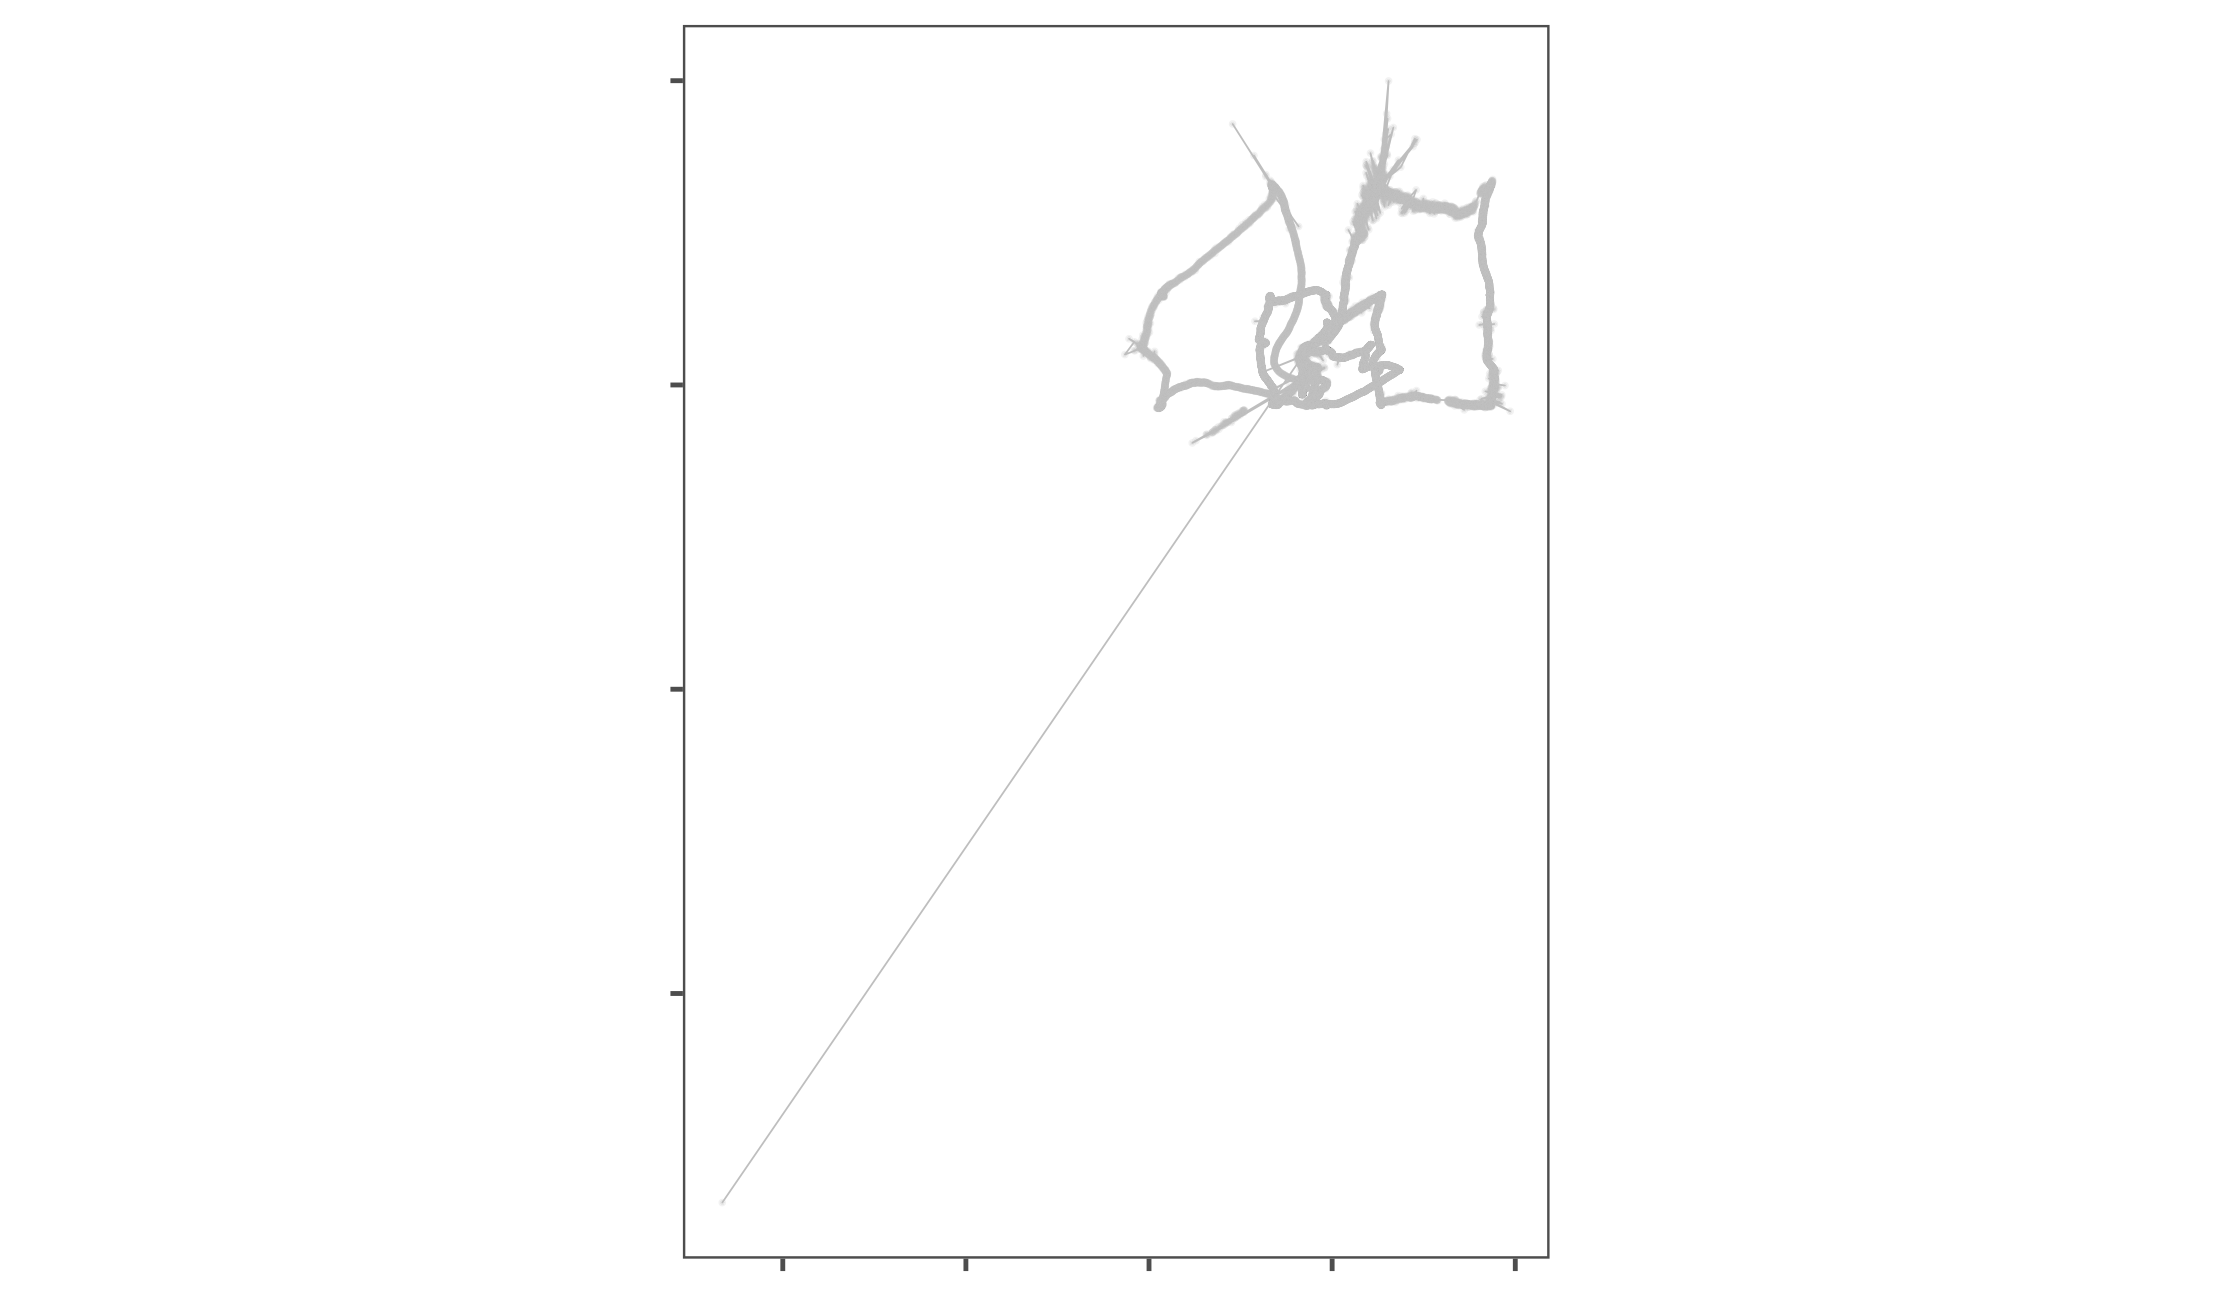
\includegraphics{figures/fig_calibration_raw.png}
\caption{The raw data from a calibration exercise conducted around the island of Griend in the Dutch Wadden Sea. A handheld WATLAS tag was used to examine how ATLAS data compared to GPS tracks, and we use the WATLAS data here to demonstrate the basics of the pre-processing pipeline, as well as validate the residence patch method. It is immediately clear from the figure that the track shows location errors, both in the form of point outliers as well as small-scale errors around the true location.}
\end{figure}

\hypertarget{filter-by-bounding-box}{%
\section{Filter by bounding box}\label{filter-by-bounding-box}}

We first save a copy of the data, so that we can plot the raw data with the cleaned data plotted over it for comparison.

\begin{Shaded}
\begin{Highlighting}[]
\CommentTok{# make a copy using the data.table copy function}
\NormalTok{data_unproc <-}\StringTok{ }\KeywordTok{copy}\NormalTok{(data)}
\end{Highlighting}
\end{Shaded}

We then filter by a bounding box in order to remove the point outlier to the far south east of the main track. We use the \texttt{atl\_filter\_bounds} functions using the \texttt{x\_range} argument, to which we pass the limit in the UTM 31N coordinate reference system.
This limit is used to exclude all points with an X coordinate \textless{} 645,000.

We then plot the result of filtering, with the excluded point in black, and the points that are retained in green.

\begin{Shaded}
\begin{Highlighting}[]
\CommentTok{# remove inside must be set to falses}
\NormalTok{data <-}\StringTok{ }\KeywordTok{atl_filter_bounds}\NormalTok{(}
  \DataTypeTok{data =}\NormalTok{ data,}
  \DataTypeTok{x =} \StringTok{"x"}\NormalTok{, }\DataTypeTok{y =} \StringTok{"y"}\NormalTok{,}
  \DataTypeTok{x_range =} \KeywordTok{c}\NormalTok{(}\DecValTok{645000}\NormalTok{, }\KeywordTok{max}\NormalTok{(data}\OperatorTok{$}\NormalTok{x)),}
  \DataTypeTok{remove_inside =} \OtherTok{FALSE}
\NormalTok{)}
\end{Highlighting}
\end{Shaded}

\begin{figure}
\centering
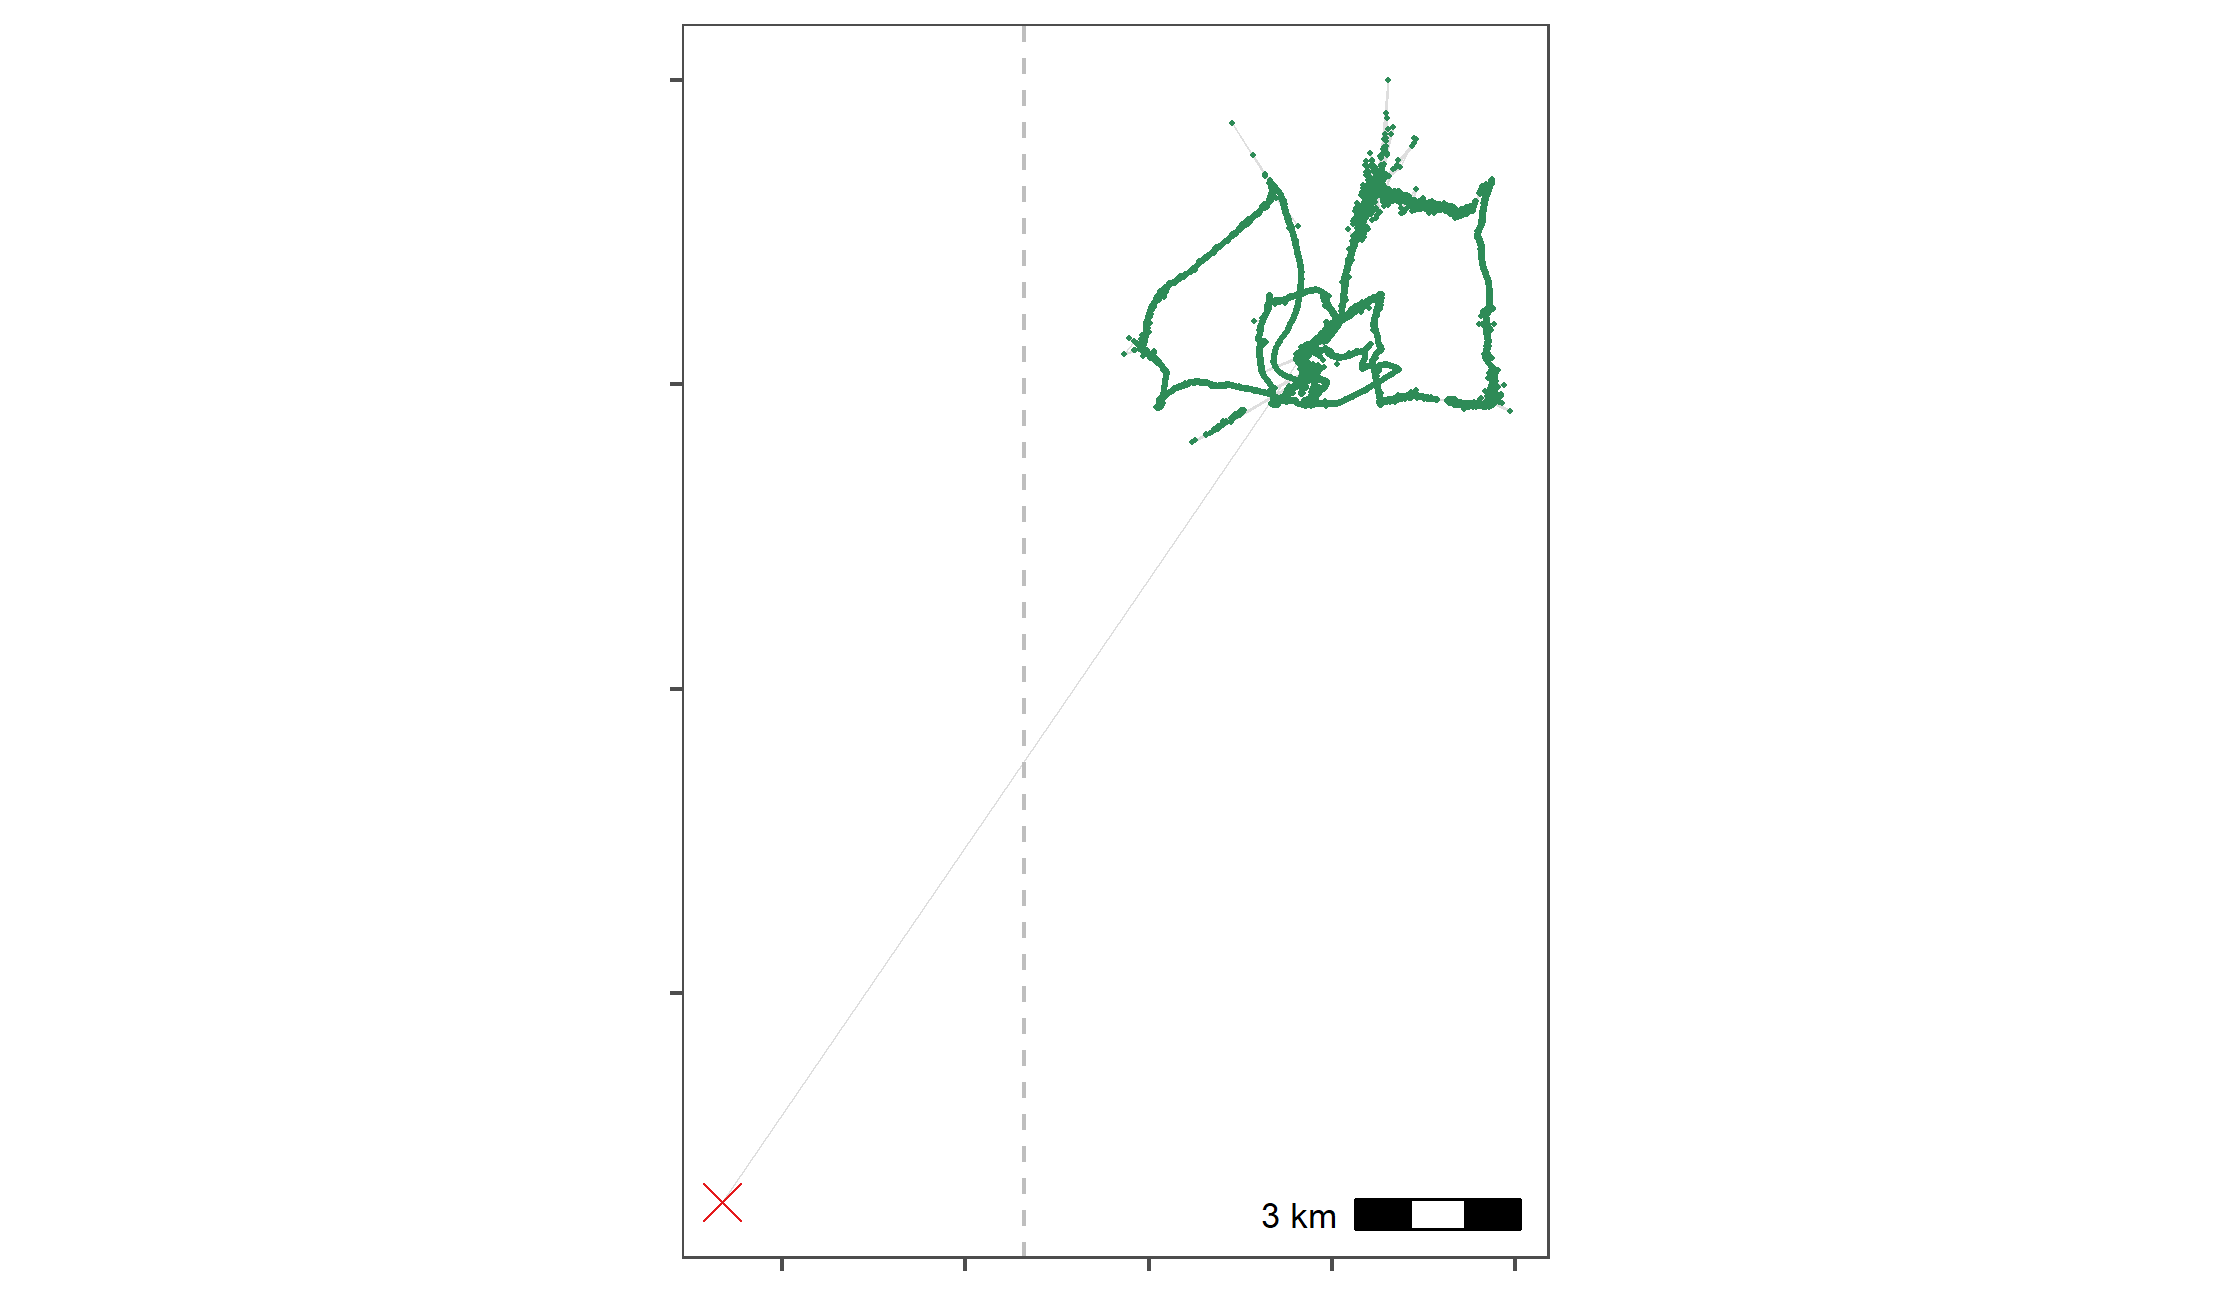
\includegraphics{figures/fig_calib_bbox.png}
\caption{Removal of a point outlier using the function \texttt{atl\_filter\_bounds}. The point outlier (black point) is removed based on its X coordinate value, with the data filtered to exclude positions with an X coordinate \textless{} 645,000 in the UTM 31N coordinate system. Positions that are retained are shown in green.}
\end{figure}

\hypertarget{filter-trajectories}{%
\section{Filter trajectories}\label{filter-trajectories}}

\hypertarget{handle-time}{%
\subsection{Handle time}\label{handle-time}}

Time in ATLAS tracks is represented by 64-bit integers (type \texttt{long}) that specify time in milliseconds, starting from the beginning of 1970 (the UNIX epoch). This representation of time is called \texttt{POSIX} time and is usually specified in seconds, not milliseconds.

Since about 1.6 billion seconds have passed since the beginning of 1970, current \texttt{POSIX} times in milliseconds cannot be represented by R's built-in 32-bit integers. A naive conversion results in truncation of out-of-range numbers leading to huge errors (dates many thousands of years in the future).

R does not natively support 64-bit integers. One option is to use the bit64 package, which adds 64-bit integer support to R.

A simpler solution is to convert the times to R's built in \texttt{double} data type (also called \texttt{numeric}), which uses a 64-bit floating point representation. This representation can represent integers with up to 16 digits without error; we only need 13 digits to represent the number of milliseconds since 1970, so the conversion is error free. We can also perform the conversion and then divide by 1000 so that times are represented in seconds, not milliseconds; this simplifies speed estimation.

If second-resolution is accurate enough (it is for our purposes), the solution that we use is to divide times by 1000 to reduce the resolution from milliseconds to seconds and then to convert the time stamps to R integers.
In the spirit of not destroying data, we create a second lower-case column called \texttt{time} to store this

\begin{Shaded}
\begin{Highlighting}[]
\CommentTok{# divide by 1000, convert to integer, then convert to POSIXct}
\NormalTok{data[, time }\OperatorTok{:}\ErrorTok{=}\StringTok{ }\KeywordTok{as.integer}\NormalTok{(}
  \KeywordTok{as.numeric}\NormalTok{(TIME) }\OperatorTok{/}\StringTok{ }\DecValTok{1000}
\NormalTok{)]}
\end{Highlighting}
\end{Shaded}

\hypertarget{add-speed-and-turning-angle}{%
\subsection{Add speed and turning angle}\label{add-speed-and-turning-angle}}

\begin{Shaded}
\begin{Highlighting}[]
\CommentTok{# add incoming and outgoing speed}
\NormalTok{data[, }\StringTok{`}\DataTypeTok{:=}\StringTok{`}\NormalTok{(}
  \DataTypeTok{speed_in =} \KeywordTok{atl_get_speed}\NormalTok{(data,}
    \DataTypeTok{x =} \StringTok{"x"}\NormalTok{,}
    \DataTypeTok{y =} \StringTok{"y"}\NormalTok{,}
    \DataTypeTok{time =} \StringTok{"time"}
\NormalTok{  ),}
  \DataTypeTok{speed_out =} \KeywordTok{atl_get_speed}\NormalTok{(data, }\DataTypeTok{type =} \StringTok{"out"}\NormalTok{)}
\NormalTok{)]}

\CommentTok{# add turning angle}
\NormalTok{data[, angle }\OperatorTok{:}\ErrorTok{=}\StringTok{ }\KeywordTok{atl_turning_angle}\NormalTok{(}\DataTypeTok{data =}\NormalTok{ data)]}
\end{Highlighting}
\end{Shaded}

\hypertarget{get-95th-percentile-of-speed-and-angle}{%
\subsection{Get 95th percentile of speed and angle}\label{get-95th-percentile-of-speed-and-angle}}

\begin{Shaded}
\begin{Highlighting}[]
\CommentTok{# use sapply}
\NormalTok{speed_angle_thresholds <-}
\StringTok{  }\KeywordTok{sapply}\NormalTok{(data[, }\KeywordTok{list}\NormalTok{(speed_in, speed_out, angle)],}
\NormalTok{    quantile,}
    \DataTypeTok{probs =} \FloatTok{0.9}\NormalTok{, }\DataTypeTok{na.rm =}\NormalTok{ T}
\NormalTok{  )}
\end{Highlighting}
\end{Shaded}

\hypertarget{filter-on-speed}{%
\subsection{Filter on speed}\label{filter-on-speed}}

Here we use a speed threshold of 15 m/s, the fastest known boat speed.
We then plot the data with the extreme speeds shown in grey, and the positions retained shown in green.

\begin{Shaded}
\begin{Highlighting}[]
\CommentTok{# make a copy}
\NormalTok{data_unproc <-}\StringTok{ }\KeywordTok{copy}\NormalTok{(data)}

\CommentTok{# remove speed outliers}
\NormalTok{data <-}\StringTok{ }\KeywordTok{atl_filter_covariates}\NormalTok{(}
  \DataTypeTok{data =}\NormalTok{ data,}
  \DataTypeTok{filters =} \KeywordTok{c}\NormalTok{(}\StringTok{"(speed_in < 15 & speed_out < 15)"}\NormalTok{)}
\NormalTok{)}

\CommentTok{# recalculate speed and angle}
\NormalTok{data[, }\StringTok{`}\DataTypeTok{:=}\StringTok{`}\NormalTok{(}
  \DataTypeTok{speed_in =} \KeywordTok{atl_get_speed}\NormalTok{(data,}
    \DataTypeTok{x =} \StringTok{"x"}\NormalTok{,}
    \DataTypeTok{y =} \StringTok{"y"}\NormalTok{,}
    \DataTypeTok{time =} \StringTok{"time"}
\NormalTok{  ),}
  \DataTypeTok{speed_out =} \KeywordTok{atl_get_speed}\NormalTok{(data, }\DataTypeTok{type =} \StringTok{"out"}\NormalTok{)}
\NormalTok{)]}

\CommentTok{# add turning angle}
\NormalTok{data[, angle }\OperatorTok{:}\ErrorTok{=}\StringTok{ }\KeywordTok{atl_turning_angle}\NormalTok{(}\DataTypeTok{data =}\NormalTok{ data)]}
\end{Highlighting}
\end{Shaded}

\begin{figure}
\centering
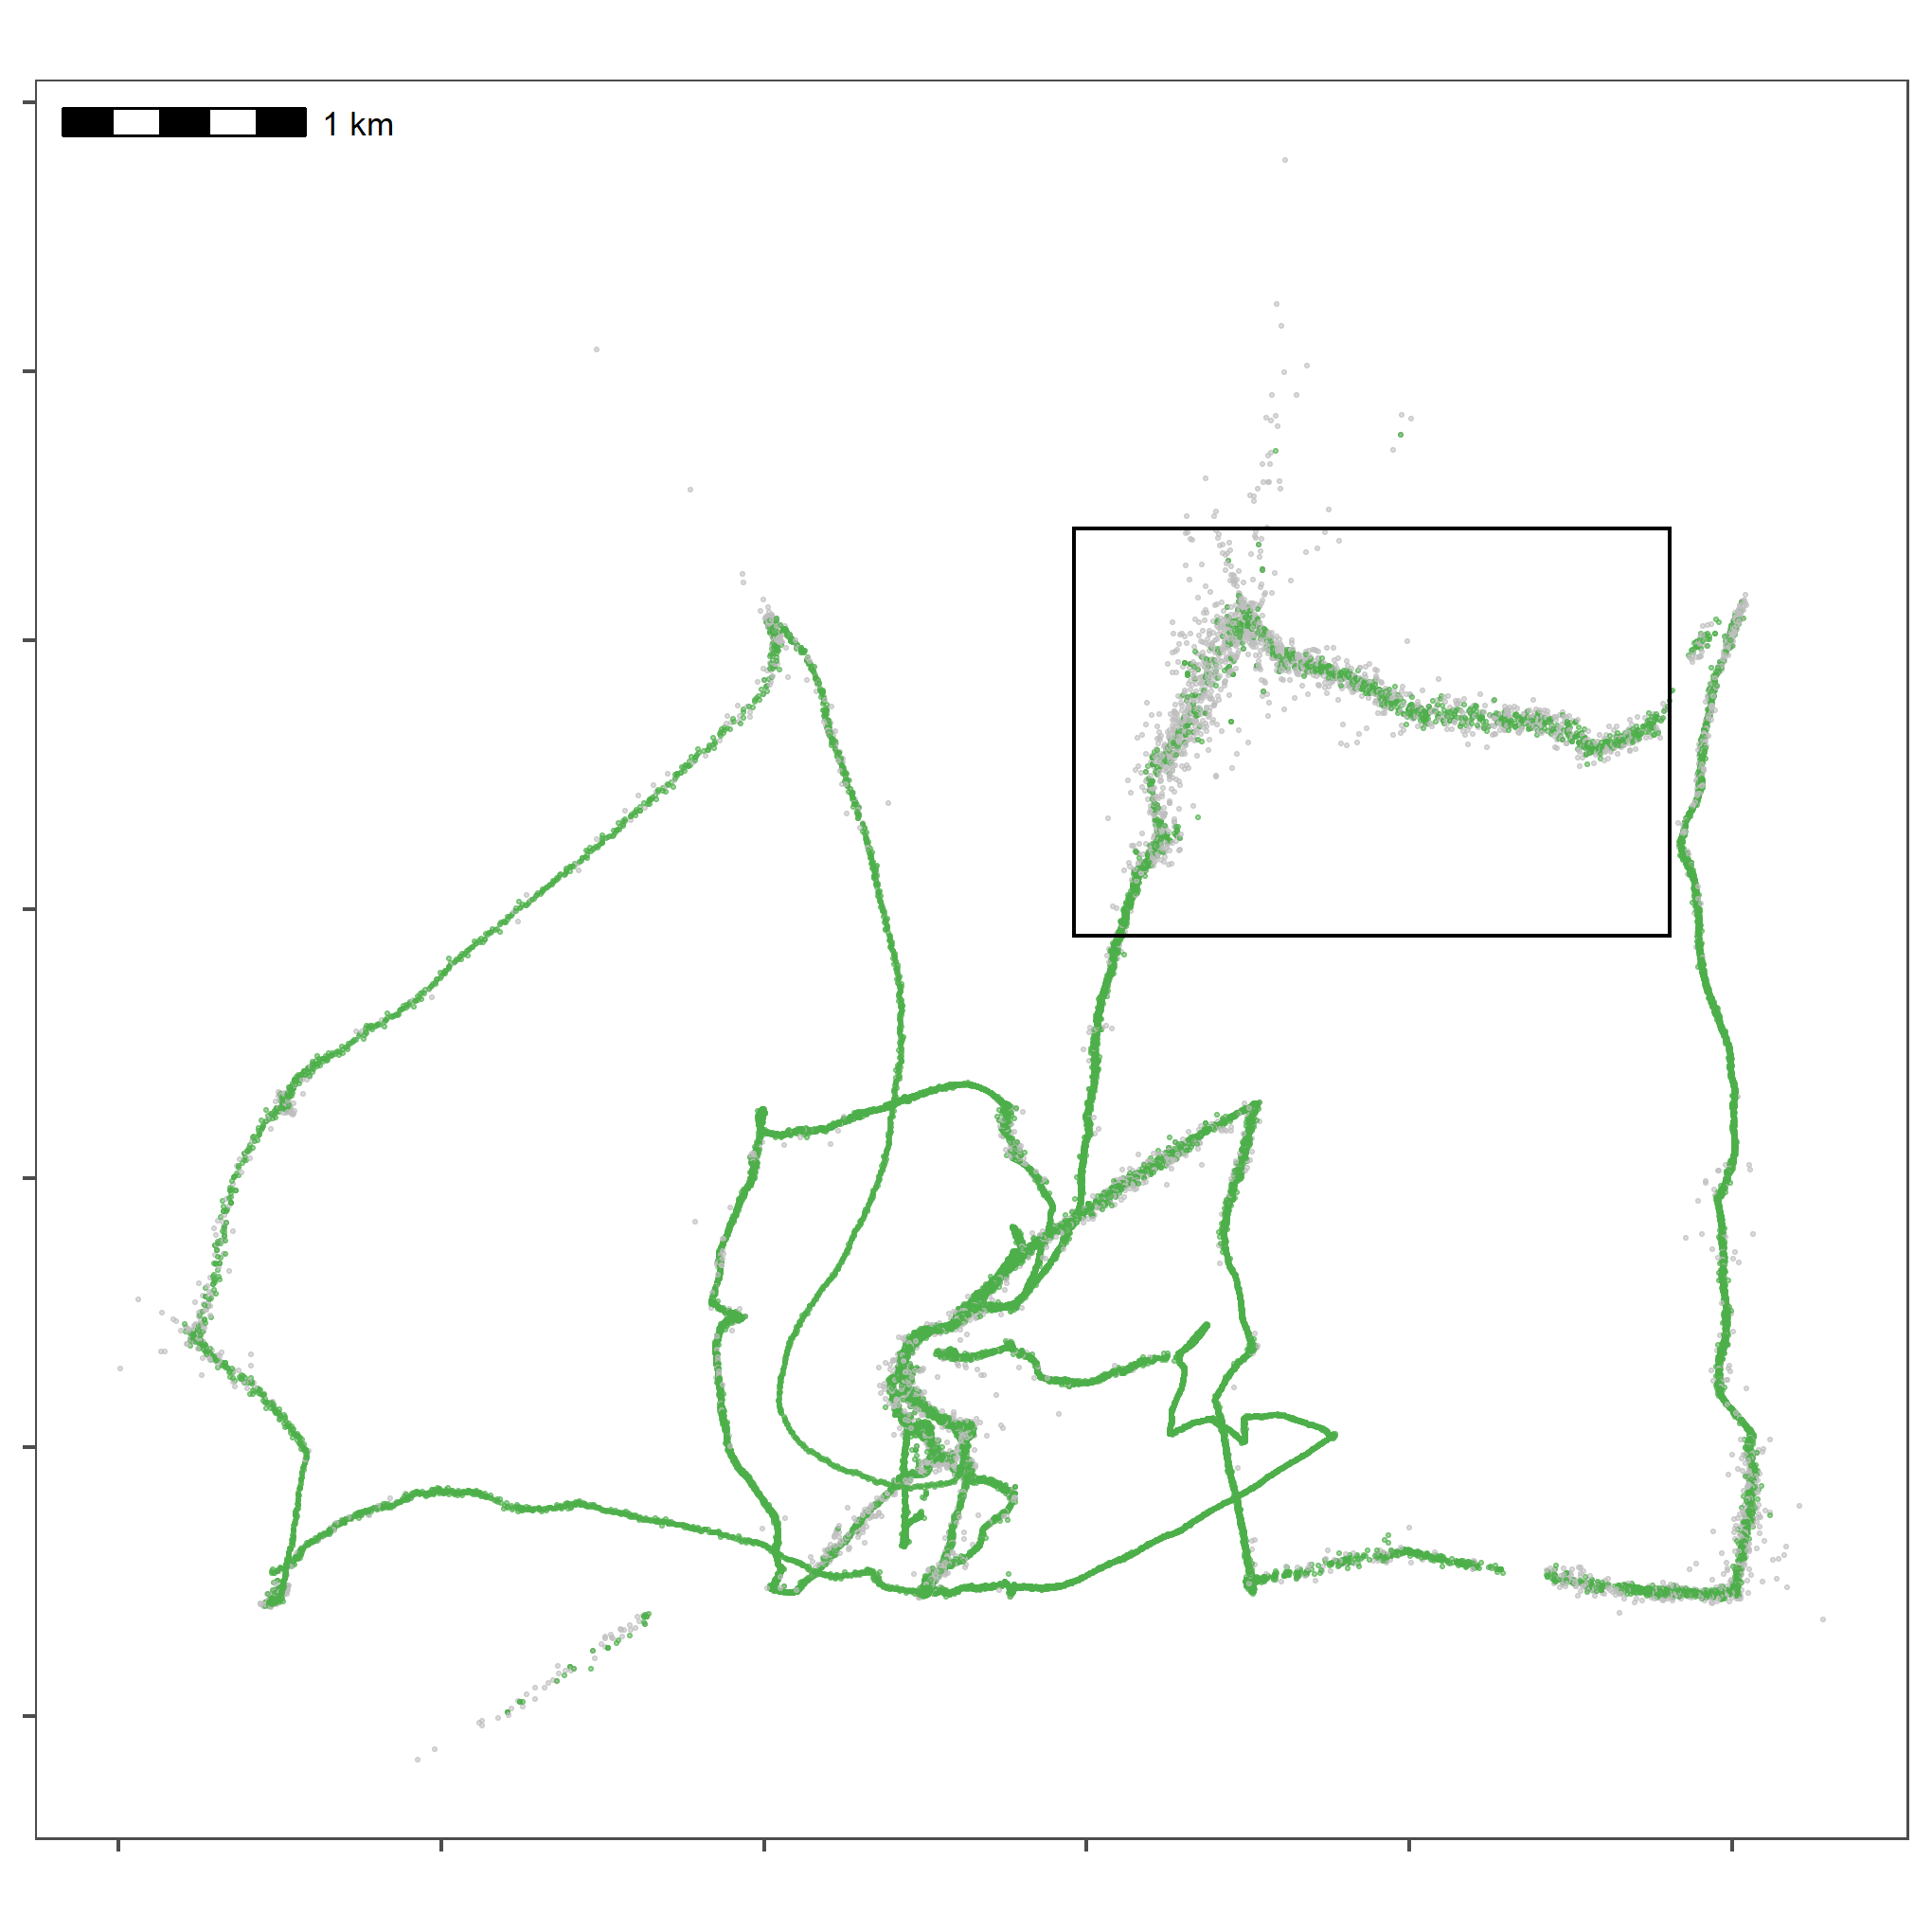
\includegraphics{figures/fig_speed_outlier.png}
\caption{Improving data quality by filtering out positions that would require unrealistic movement. We removed positions with speeds \(\geq\) 15 m/s, which is the fastest possible speed in this calibration data, part of which was collected in a moving boat around Griend. Grey positions are removed, while green positions are retained. Rectangles indicate areas expanded for visualisation in following figures.}
\end{figure}

\hypertarget{smoothing-the-trajectory}{%
\section{Smoothing the trajectory}\label{smoothing-the-trajectory}}

We then apply a median smooth over a moving window (\(K\) = 5).
This function modifies in place, and does not need to be assigned to a new variable.
We create a copy of the data before applying the smooth so that we can compare the data before and after smoothing.

\begin{Shaded}
\begin{Highlighting}[]
\CommentTok{# apply a 5 point median smooth, first make a copy}
\NormalTok{data_unproc <-}\StringTok{ }\KeywordTok{copy}\NormalTok{(data)}

\CommentTok{# now apply the smooth}
\KeywordTok{atl_median_smooth}\NormalTok{(}
  \DataTypeTok{data =}\NormalTok{ data,}
  \DataTypeTok{x =} \StringTok{"x"}\NormalTok{, }\DataTypeTok{y =} \StringTok{"y"}\NormalTok{, }\DataTypeTok{time =} \StringTok{"time"}\NormalTok{,}
  \DataTypeTok{moving_window =} \DecValTok{5}
\NormalTok{)}
\end{Highlighting}
\end{Shaded}

\begin{figure}
\centering
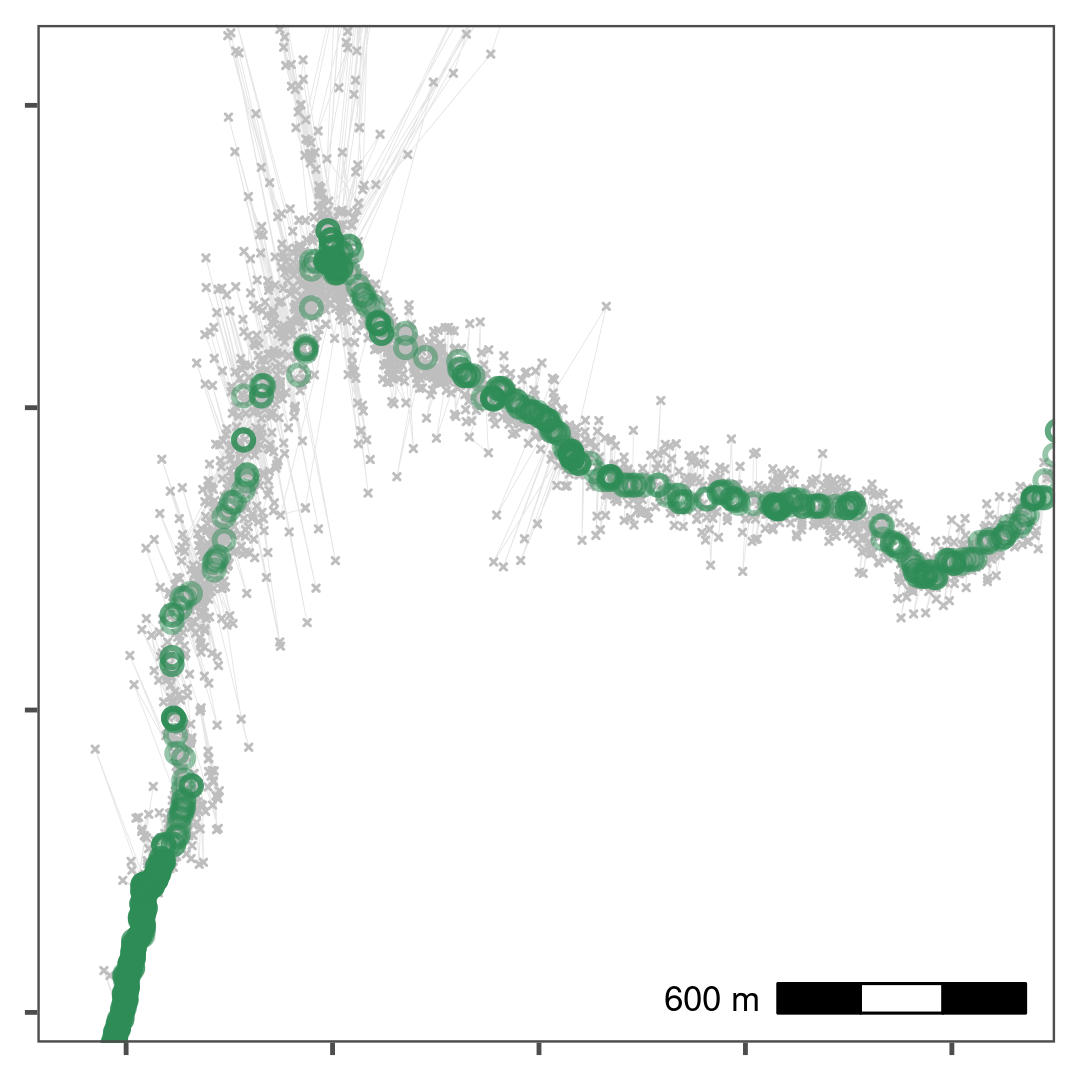
\includegraphics{figures/fig_calib_median_smooth.png}
\caption{Reducing small-scale location error using a median smooth with a moving window \(K\) = 5. Median smoothed positions are shown in green, while raw, unfiltered data is shown in grey. Median smoothing successfully recovers the likely path of the track without a loss of data. The area shown is the upper rectangle from Fig. 1.3.}
\end{figure}

\hypertarget{thinning-the-data}{%
\section{Thinning the data}\label{thinning-the-data}}

Next we thin the data to demonstrate thinning by median smoothing.
Following this, we plot the median smooth and thinning by aggregation.

\begin{Shaded}
\begin{Highlighting}[]
\CommentTok{# save a copy}
\NormalTok{data_unproc <-}\StringTok{ }\KeywordTok{copy}\NormalTok{(data)}

\CommentTok{# remove columns we don't need}
\NormalTok{data <-}\StringTok{ }\NormalTok{data[, }\KeywordTok{setdiff}\NormalTok{(}
  \KeywordTok{colnames}\NormalTok{(data),}
  \KeywordTok{c}\NormalTok{(}\StringTok{"tID"}\NormalTok{, }\StringTok{"Timestamp"}\NormalTok{, }\StringTok{"id"}\NormalTok{, }\StringTok{"TIME"}\NormalTok{, }\StringTok{"UTCtime"}\NormalTok{)}
\NormalTok{),}
\NormalTok{with =}\StringTok{ }\OtherTok{FALSE}
\NormalTok{]}

\CommentTok{# thin to a 30s interval}
\NormalTok{data_thin <-}\StringTok{ }\KeywordTok{atl_thin_data}\NormalTok{(}
  \DataTypeTok{data =}\NormalTok{ data,}
  \DataTypeTok{interval =} \DecValTok{30}\NormalTok{,}
  \DataTypeTok{method =} \StringTok{"aggregate"}\NormalTok{,}
  \DataTypeTok{id_columns =} \StringTok{"TAG"}
\NormalTok{)}
\end{Highlighting}
\end{Shaded}

\begin{figure}
\centering
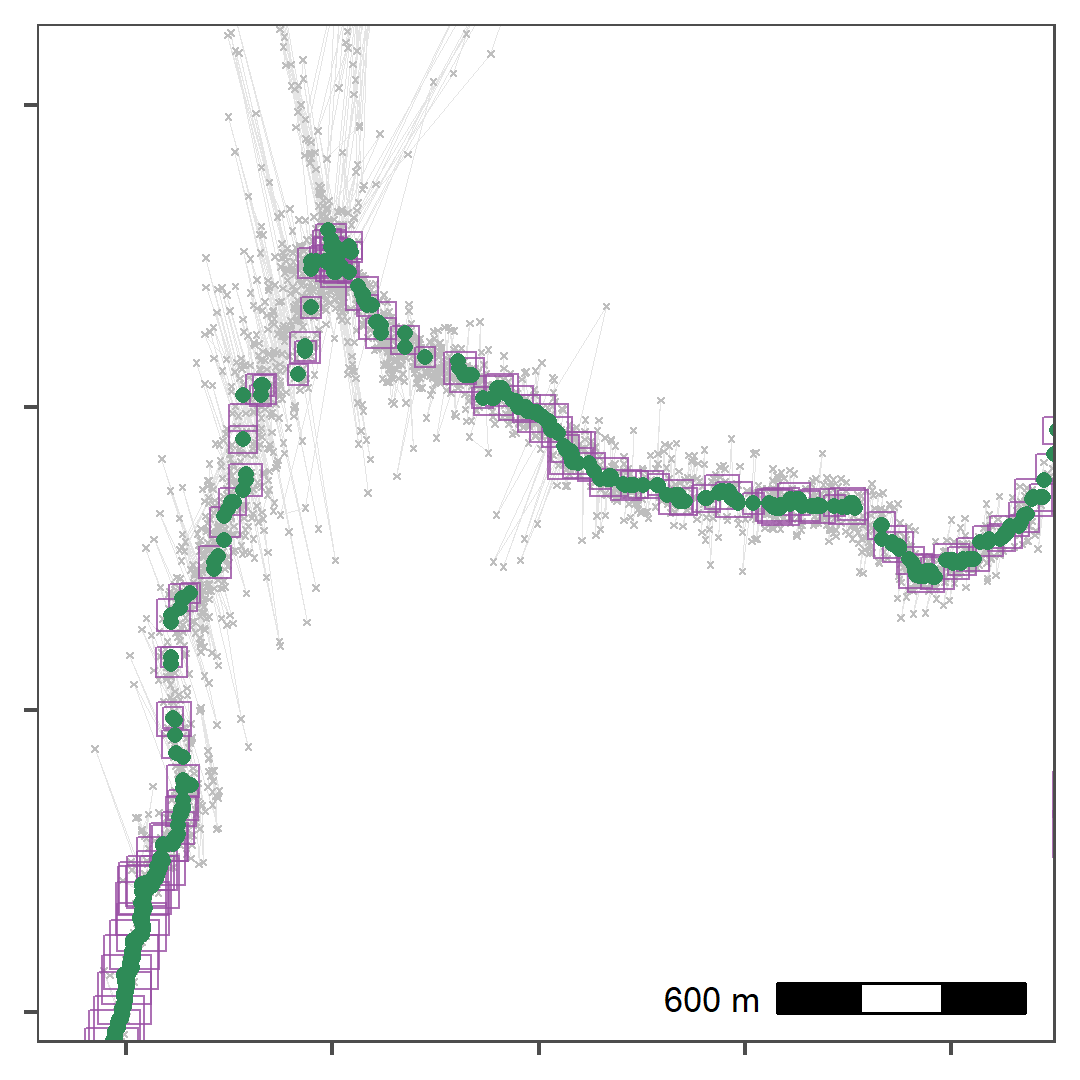
\includegraphics{figures/fig_calib_smooth_thin.png}
\caption{Thinning by aggregation over a 30 second interval (down from 1 second) preserves track structure while reducing the data volume for computation. Here, thinned positions are shown as purple squares, with the size of the square indicating the number of positions within the 30 second bin used to obtain the average position. Green points show the median smoothed data from Fig. 1.4, while the raw data are shown in grey. The area shown is the upper rectangle in Fig. 1.3.}
\end{figure}

\hypertarget{residence-patches}{%
\section{Residence patches}\label{residence-patches}}

\hypertarget{get-waypoint-centroids}{%
\subsection{Get waypoint centroids}\label{get-waypoint-centroids}}

We subset the annotated calibration data to select the waypoints and the positions around them which are supposed to be the locations of known stops. Since each stop was supposed to be 5 minutes long, there are multiple points in each known stop.

\begin{Shaded}
\begin{Highlighting}[]
\KeywordTok{library}\NormalTok{(stringi)}
\NormalTok{data_res <-}\StringTok{ }\NormalTok{data_unproc[}\KeywordTok{stri_detect}\NormalTok{(tID, }\DataTypeTok{regex =} \StringTok{"(WP)"}\NormalTok{)]}
\end{Highlighting}
\end{Shaded}

From this data, we get the centroid of known stops, and determine the time difference between the first and last point within 50 metres, and within 10 minutes of the waypoint positions' median time.

Essentially, this means that the maximum duration of a stop can be 20 minutes, and stops above this duration are not expected.

\begin{Shaded}
\begin{Highlighting}[]
\CommentTok{# get centroid}
\NormalTok{data_res_summary <-}\StringTok{ }\NormalTok{data_res[, }\KeywordTok{list}\NormalTok{(}
  \DataTypeTok{x_median =} \KeywordTok{median}\NormalTok{(x),}
  \DataTypeTok{y_median =} \KeywordTok{median}\NormalTok{(y),}
  \DataTypeTok{t_median =} \KeywordTok{median}\NormalTok{(time)}
\NormalTok{),}
\NormalTok{by =}\StringTok{ "tID"}
\NormalTok{]}

\CommentTok{# now get times 10 mins before and after}
\NormalTok{data_res_summary[, }\StringTok{`}\DataTypeTok{:=}\StringTok{`}\NormalTok{(}
  \DataTypeTok{t_min =}\NormalTok{ t_median }\OperatorTok{-}\StringTok{ }\NormalTok{(}\DecValTok{10} \OperatorTok{*}\StringTok{ }\DecValTok{60}\NormalTok{),}
  \DataTypeTok{t_max =}\NormalTok{ t_median }\OperatorTok{+}\StringTok{ }\NormalTok{(}\DecValTok{10} \OperatorTok{*}\StringTok{ }\DecValTok{60}\NormalTok{)}
\NormalTok{)]}

\CommentTok{# make a list of positions 10min before and after}
\NormalTok{wp_data <-}\StringTok{ }\KeywordTok{mapply}\NormalTok{(}\ControlFlowTok{function}\NormalTok{(l, u, mx, my) \{}
\NormalTok{  tmp_data <-}\StringTok{ }\NormalTok{data_unproc[}\KeywordTok{inrange}\NormalTok{(time, l, u)]}
\NormalTok{  tmp_data[, distance }\OperatorTok{:}\ErrorTok{=}\StringTok{ }\KeywordTok{sqrt}\NormalTok{((mx }\OperatorTok{-}\StringTok{ }\NormalTok{x)}\OperatorTok{^}\DecValTok{2} \OperatorTok{+}\StringTok{ }\NormalTok{(my }\OperatorTok{-}\StringTok{ }\NormalTok{y)}\OperatorTok{^}\DecValTok{2}\NormalTok{)]}

  \CommentTok{# keep within 50}
\NormalTok{  tmp_data <-}\StringTok{ }\NormalTok{tmp_data[distance }\OperatorTok{<=}\StringTok{ }\DecValTok{50}\NormalTok{, ]}

  \CommentTok{# get duration}
  \KeywordTok{return}\NormalTok{(}\KeywordTok{diff}\NormalTok{(}\KeywordTok{range}\NormalTok{(tmp_data}\OperatorTok{$}\NormalTok{time)))}
\NormalTok{\}, data_res_summary}\OperatorTok{$}\NormalTok{t_min, data_res_summary}\OperatorTok{$}\NormalTok{t_max,}
\NormalTok{data_res_summary}\OperatorTok{$}\NormalTok{x_median, data_res_summary}\OperatorTok{$}\NormalTok{y_median,}
\DataTypeTok{SIMPLIFY =} \OtherTok{TRUE}
\NormalTok{)}
\end{Highlighting}
\end{Shaded}

\hypertarget{prepare-data}{%
\subsection{Prepare data}\label{prepare-data}}

An indicator of individual residence at or near a position can be useful when attempting to identify residence patches. Positions can be filtered on a metric such as residence time (Bracis, Bildstein, and Mueller \protect\hyperlink{ref-bracis2018}{2018}).

\hypertarget{calculate-residence-time}{%
\subsection{Calculate residence time}\label{calculate-residence-time}}

First we calculate the residence time with a radius of 50 metres.
For this, we need a dataframe with coordinates, the timestamp, and the animal id.
We save this data to file for later use.

\begin{Shaded}
\begin{Highlighting}[]
\CommentTok{# get 4 column data}
\NormalTok{data_for_patch <-}\StringTok{ }\NormalTok{data_thin[, }\KeywordTok{list}\NormalTok{(x, y, time, TAG)]}

\CommentTok{# get recurse data for a 10m radius}
\NormalTok{recurse_stats <-}\StringTok{ }\KeywordTok{getRecursions}\NormalTok{(data_for_patch,}
  \DataTypeTok{radius =} \DecValTok{50}\NormalTok{, }\DataTypeTok{timeunits =} \StringTok{"mins"}
\NormalTok{)}

\CommentTok{# assign to recurse data}
\NormalTok{data_for_patch[, res_time }\OperatorTok{:}\ErrorTok{=}\StringTok{ }\NormalTok{recurse_stats}\OperatorTok{$}\NormalTok{residenceTime]}

\CommentTok{# save recurse data}
\KeywordTok{fwrite}\NormalTok{(data_for_patch, }\DataTypeTok{file =} \StringTok{"data/data_calib_for_patch.csv"}\NormalTok{)}
\end{Highlighting}
\end{Shaded}

\hypertarget{run-residence-patch-method}{%
\subsection{Run residence patch method}\label{run-residence-patch-method}}

We subset data with a residence time \textgreater{} 5 minutes in order to construct residence patches.
From this subset, we construct residence patches using the parameters: \texttt{buffer\_radius} = 5 metres, \texttt{lim\_spat\_indep} = 50 metres, \texttt{lim\_time\_indep} = 5 minutes, and \texttt{min\_fixes} = 3.

\begin{Shaded}
\begin{Highlighting}[]
\CommentTok{# assign id as tag}
\NormalTok{data_for_patch[, id }\OperatorTok{:}\ErrorTok{=}\StringTok{ }\KeywordTok{as.character}\NormalTok{(TAG)]}

\CommentTok{# on known residence points}
\NormalTok{patch_res_known <-}\StringTok{ }\KeywordTok{atl_res_patch}\NormalTok{(data_for_patch[res_time }\OperatorTok{>=}\StringTok{ }\DecValTok{5}\NormalTok{, ],}
  \DataTypeTok{buffer_radius =} \DecValTok{5}\NormalTok{,}
  \DataTypeTok{lim_spat_indep =} \DecValTok{50}\NormalTok{,}
  \DataTypeTok{lim_time_indep =} \DecValTok{5}\NormalTok{,}
  \DataTypeTok{min_fixes =} \DecValTok{3}
\NormalTok{)}
\end{Highlighting}
\end{Shaded}

\hypertarget{get-spatial-and-summary-objects}{%
\subsection{Get spatial and summary objects}\label{get-spatial-and-summary-objects}}

We get spatial and summary ouput of the residence patch method using the \texttt{atl\_patch\_summary} function using the options \texttt{which\_data} = ``spatial'' and \texttt{which\_data} = "summary.
We use a buffer radius here of 20 metres for the spatial buffer, despite using a buffer radius of 5 metres earlier, simply because it is easier to visualise in the output figure.

\begin{Shaded}
\begin{Highlighting}[]
\CommentTok{# for the known and unkniwn patches}
\NormalTok{patch_sf_data <-}\StringTok{ }\KeywordTok{atl_patch_summary}\NormalTok{(patch_res_known,}
  \DataTypeTok{which_data =} \StringTok{"spatial"}\NormalTok{,}
  \DataTypeTok{buffer_radius =} \DecValTok{20}
\NormalTok{)}

\CommentTok{# assign crs}
\NormalTok{sf}\OperatorTok{::}\KeywordTok{st_crs}\NormalTok{(patch_sf_data) <-}\StringTok{ }\DecValTok{32631}

\CommentTok{# get summary data}
\NormalTok{patch_summary_data <-}\StringTok{ }\KeywordTok{atl_patch_summary}\NormalTok{(patch_res_known,}
  \DataTypeTok{which_data =} \StringTok{"summary"}
\NormalTok{)}
\end{Highlighting}
\end{Shaded}

\hypertarget{prepare-to-plot-data}{%
\subsection{Prepare to plot data}\label{prepare-to-plot-data}}

We read in the island's shapefile to plot it as a background for the residence patch figure.

\begin{Shaded}
\begin{Highlighting}[]
\CommentTok{# read griend and hut}
\NormalTok{griend <-}\StringTok{ }\NormalTok{sf}\OperatorTok{::}\KeywordTok{st_read}\NormalTok{(}\StringTok{"data/griend_polygon/griend_polygon.shp"}\NormalTok{)}
\NormalTok{hut <-}\StringTok{ }\NormalTok{sf}\OperatorTok{::}\KeywordTok{st_read}\NormalTok{(}\StringTok{"data/griend_hut.gpkg"}\NormalTok{)}
\end{Highlighting}
\end{Shaded}

\begin{figure}
\centering
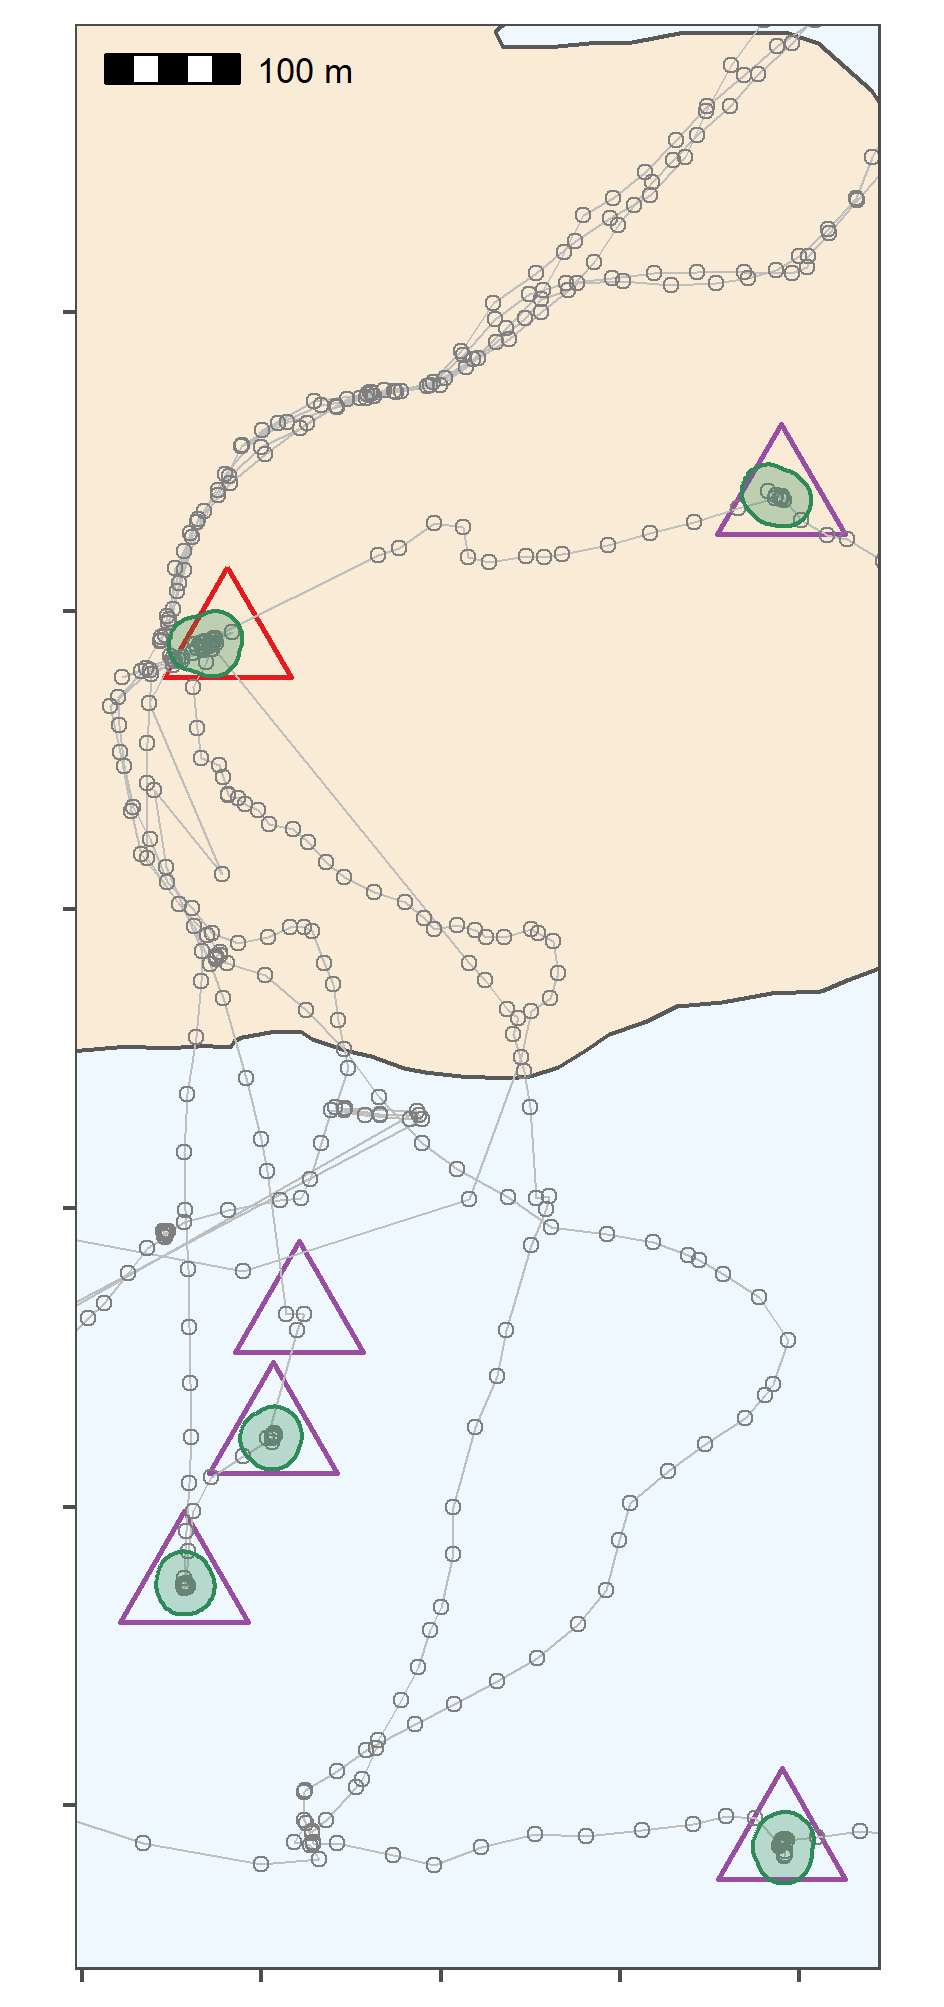
\includegraphics{figures/fig_calib_residence.png}
\caption{Classifying thinned data into residence patches yields robust estimates of the duration of known stops. The island of Griend (53.25\(^{\circ}\)N, 5.25\(^{\circ}\)E) is shown in beige. Residence patches (green polygons; function parameters in text) correspond well to the locations of known stops (purple triangles). However, the algorithm identified all areas with prolonged residence, including those which were not intended stops (n = 12; green polygons without triangles). The algorithm also failed to find two stops of 6 and 15 seconds duration, since these were lost in the data thinning step (triangle without green polygon shows one of these). The area shown is the lower rectangle in Fig. 1.3.}
\end{figure}

\hypertarget{compare-patch-metrics}{%
\section{Compare patch metrics}\label{compare-patch-metrics}}

We then merge the annoated, known stop data with the calculated patch duration.
We filter this data to exclude one exceedingly long outlier of about an hour (WP080), which how

\begin{Shaded}
\begin{Highlighting}[]
\CommentTok{# get known patch summary}
\NormalTok{data_res <-}\StringTok{ }\NormalTok{data_unproc[stringi}\OperatorTok{::}\KeywordTok{stri_detect}\NormalTok{(tID, }\DataTypeTok{regex =} \StringTok{"(WP)"}\NormalTok{), ]}

\CommentTok{# get waypoint summary}
\NormalTok{patch_summary_real <-}\StringTok{ }\NormalTok{data_res[, }\KeywordTok{list}\NormalTok{(}
  \DataTypeTok{nfixes_real =}\NormalTok{ .N,}
  \DataTypeTok{x_median =} \KeywordTok{round}\NormalTok{(}\KeywordTok{median}\NormalTok{(x), }\DataTypeTok{digits =} \DecValTok{-2}\NormalTok{),}
  \DataTypeTok{y_median =} \KeywordTok{round}\NormalTok{(}\KeywordTok{median}\NormalTok{(y), }\DataTypeTok{digits =} \DecValTok{-2}\NormalTok{)}
\NormalTok{),}
\NormalTok{by =}\StringTok{ "tID"}
\NormalTok{]}

\CommentTok{# add real duration}
\NormalTok{patch_summary_real[, duration_real }\OperatorTok{:}\ErrorTok{=}\StringTok{ }\NormalTok{wp_data]}

\CommentTok{# round median coordinate for inferred patches}
\NormalTok{patch_summary_inferred <-}
\StringTok{  }\NormalTok{patch_summary_data[}
\NormalTok{    ,}
    \KeywordTok{c}\NormalTok{(}
      \StringTok{"x_median"}\NormalTok{, }\StringTok{"y_median"}\NormalTok{,}
      \StringTok{"nfixes"}\NormalTok{, }\StringTok{"duration"}\NormalTok{, }\StringTok{"patch"}
\NormalTok{    )}
\NormalTok{  ][, }\StringTok{`}\DataTypeTok{:=}\StringTok{`}\NormalTok{(}
    \DataTypeTok{x_median =} \KeywordTok{round}\NormalTok{(x_median, }\DataTypeTok{digits =} \DecValTok{-2}\NormalTok{),}
    \DataTypeTok{y_median =} \KeywordTok{round}\NormalTok{(y_median, }\DataTypeTok{digits =} \DecValTok{-2}\NormalTok{)}
\NormalTok{  )]}

\CommentTok{# join with respatch summary}
\NormalTok{patch_summary_compare <-}
\StringTok{  }\KeywordTok{merge}\NormalTok{(patch_summary_real,}
\NormalTok{    patch_summary_inferred,}
    \DataTypeTok{on =} \KeywordTok{c}\NormalTok{(}\StringTok{"x_median"}\NormalTok{, }\StringTok{"y_median"}\NormalTok{),}
    \DataTypeTok{all.x =} \OtherTok{TRUE}\NormalTok{, }\DataTypeTok{all.y =} \OtherTok{TRUE}
\NormalTok{  )}

\CommentTok{# drop nas}
\NormalTok{patch_summary_compare <-}\StringTok{ }\KeywordTok{na.omit}\NormalTok{(patch_summary_compare)}

\CommentTok{# drop patch around WP080}
\NormalTok{patch_summary_compare <-}\StringTok{ }\NormalTok{patch_summary_compare[tID }\OperatorTok{!=}\StringTok{ "WP080"}\NormalTok{, ]}
\end{Highlighting}
\end{Shaded}

7 patches are identified where there are no waypoints, while 2 waypoints are not identified as patches. These waypoints consisted of 6 and 15 (WP098 and WP092) positions respectively, and were lost when the data were aggregated to 30 second intervals.

\hypertarget{linear-model-durations}{%
\subsection{Linear model durations}\label{linear-model-durations}}

We run a simple linear model.

\begin{Shaded}
\begin{Highlighting}[]
\CommentTok{# get linear model}
\NormalTok{model_duration <-}\StringTok{ }\KeywordTok{lm}\NormalTok{(duration_real }\OperatorTok{~}\StringTok{ }\NormalTok{duration,}
  \DataTypeTok{data =}\NormalTok{ patch_summary_compare}
\NormalTok{)}

\CommentTok{# get R2}
\KeywordTok{summary}\NormalTok{(model_duration)}

\CommentTok{# write to file}
\KeywordTok{writeLines}\NormalTok{(}
  \DataTypeTok{text =} \KeywordTok{capture.output}\NormalTok{(}
    \KeywordTok{summary}\NormalTok{(model_duration)}
\NormalTok{  ),}
  \DataTypeTok{con =} \StringTok{"data/model_output_residence_patch.txt"}
\NormalTok{)}
\end{Highlighting}
\end{Shaded}

\begin{figure}
\centering
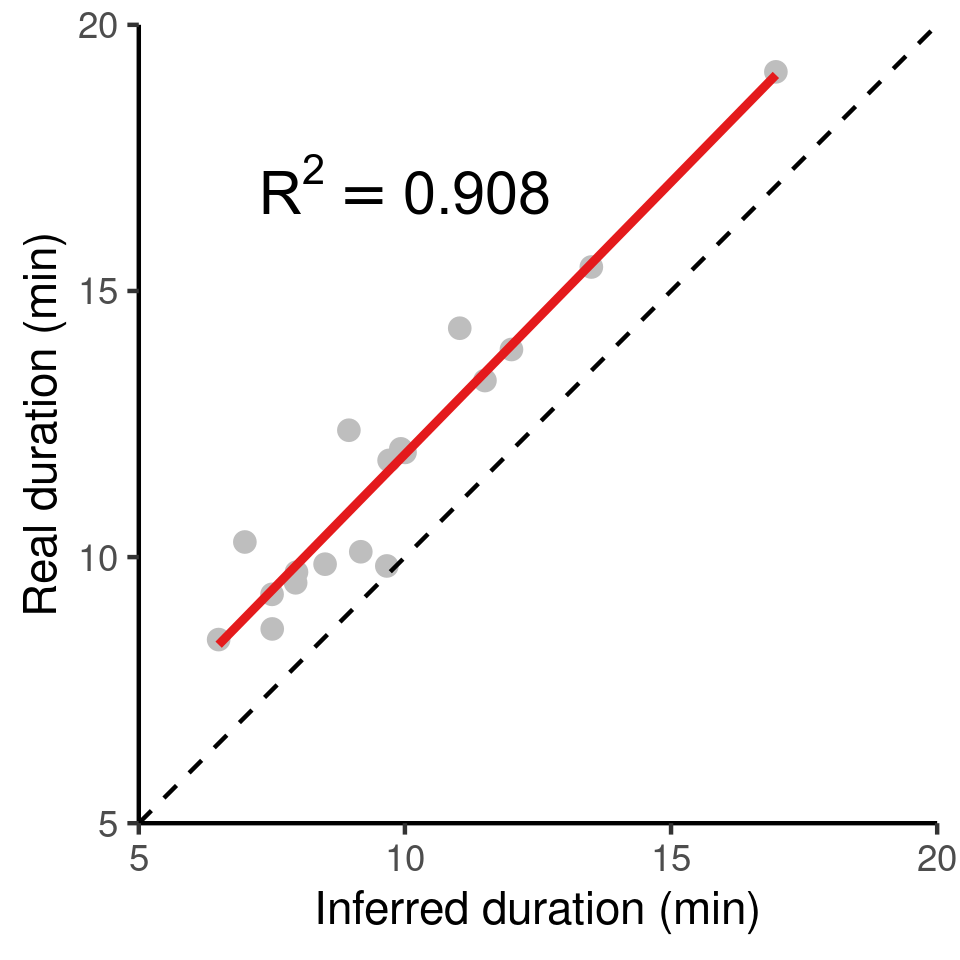
\includegraphics{figures/fig_calib_lm_duration.png}
\caption{The inferred duration of residence patches corresponds very closely to the real duration (grey circles, red line shows linear model fit), with an underestimation of the true duration of around 2\%. The dashed black line represents \(y = x\) for reference.}
\end{figure}

\hypertarget{linear-model-summary}{%
\subsection{Linear model summary}\label{linear-model-summary}}

\begin{Shaded}
\begin{Highlighting}[]
\KeywordTok{cat}\NormalTok{(}
  \KeywordTok{readLines}\NormalTok{(}
    \DataTypeTok{con =} \StringTok{"data/model_output_residence_patch.txt"}\NormalTok{,}
    \DataTypeTok{encoding =} \StringTok{"UTF-8"}
\NormalTok{  ),}
  \DataTypeTok{sep =} \StringTok{"}\CharTok{\textbackslash{}n}\StringTok{"}
\NormalTok{)}
\CommentTok{#> }
\CommentTok{#> Call:}
\CommentTok{#> lm(formula = duration_real ~ duration, data = patch_summary_compare)}
\CommentTok{#> }
\CommentTok{#> Residuals:}
\CommentTok{#>      Min       1Q   Median       3Q      Max }
\CommentTok{#> -103.237  -19.277   -2.917    7.003   93.431 }
\CommentTok{#> }
\CommentTok{#> Coefficients:}
\CommentTok{#>              Estimate Std. Error t value Pr(>|t|)    }
\CommentTok{#> (Intercept) 101.42061   47.66936   2.128   0.0493 *  }
\CommentTok{#> duration      1.02108    0.07876  12.965 6.66e-10 ***}
\CommentTok{#> ---}
\CommentTok{#> Signif. codes:  0 ‘***’ 0.001 ‘**’ 0.01 ‘*’ 0.05 ‘.’ 0.1 ‘ ’ 1}
\CommentTok{#> }
\CommentTok{#> Residual standard error: 50.35 on 16 degrees of freedom}
\CommentTok{#> Multiple R-squared:  0.9131, Adjusted R-squared:  0.9077 }
\CommentTok{#> F-statistic: 168.1 on 1 and 16 DF,  p-value: 6.655e-10}
\end{Highlighting}
\end{Shaded}

\hypertarget{plot-figure-7}{%
\section{Plot figure 7}\label{plot-figure-7}}

Plotting code is not shown in PDF and HTML form, see the \texttt{.Rmd} file.

\hypertarget{processing-egyptian-fruit-bat-tracks}{%
\chapter{Processing Egyptian Fruit Bat Tracks}\label{processing-egyptian-fruit-bat-tracks}}

We show the pre-processing pipeline at work on the tracks of three Egyptian fruit bats (\emph{Rousettus aegyptiacus}), and construct residence patches.

\hypertarget{prepare-libraries-1}{%
\section{Prepare libraries}\label{prepare-libraries-1}}

Install the required \texttt{R} libraries that are required from CRAN if not already installed.

\begin{Shaded}
\begin{Highlighting}[]
\CommentTok{# libs for data}
\KeywordTok{library}\NormalTok{(data.table)}
\KeywordTok{library}\NormalTok{(RSQLite)}
\KeywordTok{library}\NormalTok{(atlastools)}

\CommentTok{# libs for plotting}
\KeywordTok{library}\NormalTok{(ggplot2)}
\KeywordTok{library}\NormalTok{(patchwork)}

\CommentTok{# recursion analysis}
\KeywordTok{library}\NormalTok{(recurse)}

\CommentTok{# prepare a palette}
\NormalTok{pal <-}\StringTok{ }\NormalTok{RColorBrewer}\OperatorTok{::}\KeywordTok{brewer.pal}\NormalTok{(}\DecValTok{4}\NormalTok{, }\StringTok{"Set1"}\NormalTok{)}
\end{Highlighting}
\end{Shaded}

\hypertarget{read-bat-data}{%
\section{Read bat data}\label{read-bat-data}}

Read the bat data from an \texttt{SQLite} database local file and convert to a plain text csv file.
This data can be found in the ``data'' folder.

\begin{Shaded}
\begin{Highlighting}[]
\CommentTok{# prepare the connection}
\NormalTok{con <-}\StringTok{ }\KeywordTok{dbConnect}\NormalTok{(}
  \DataTypeTok{drv =} \KeywordTok{SQLite}\NormalTok{(),}
  \DataTypeTok{dbname =} \StringTok{"data/Three_example_bats.sql"}
\NormalTok{)}

\CommentTok{# list the tables}
\NormalTok{table_name <-}\StringTok{ }\KeywordTok{dbListTables}\NormalTok{(con)}

\CommentTok{# prepare to query all tables}
\NormalTok{query <-}\StringTok{ }\KeywordTok{sprintf}\NormalTok{(}\StringTok{'select * from }\CharTok{\textbackslash{}"}\StringTok{%s}\CharTok{\textbackslash{}"}\StringTok{'}\NormalTok{, table_name)}

\CommentTok{# query the database}
\NormalTok{data <-}\StringTok{ }\KeywordTok{dbGetQuery}\NormalTok{(}\DataTypeTok{conn =}\NormalTok{ con, }\DataTypeTok{statement =}\NormalTok{ query)}

\CommentTok{# disconnect from database}
\KeywordTok{dbDisconnect}\NormalTok{(con)}
\end{Highlighting}
\end{Shaded}

Convert data to csv, and save a local copy in the folder ``data''.

\begin{Shaded}
\begin{Highlighting}[]
\CommentTok{# convert data to datatable}
\KeywordTok{setDT}\NormalTok{(data)}

\CommentTok{# write data for QGIS}
\KeywordTok{fwrite}\NormalTok{(data, }\DataTypeTok{file =} \StringTok{"data/bat_data.csv"}\NormalTok{)}
\end{Highlighting}
\end{Shaded}

\hypertarget{a-first-visual-inspection}{%
\section{A First Visual Inspection}\label{a-first-visual-inspection}}

Plot the bat data as a sanity check, and inspect it visually for errors (Fig. 2.1).
The plot code is hidden in the rendered copy (PDF) of this supplementary material, but is available in the \texttt{Rmarkdown} file ``06\_bat\_data.Rmd''.
The saved plot is shown below as Fig. 2.1.

\begin{figure}
\centering
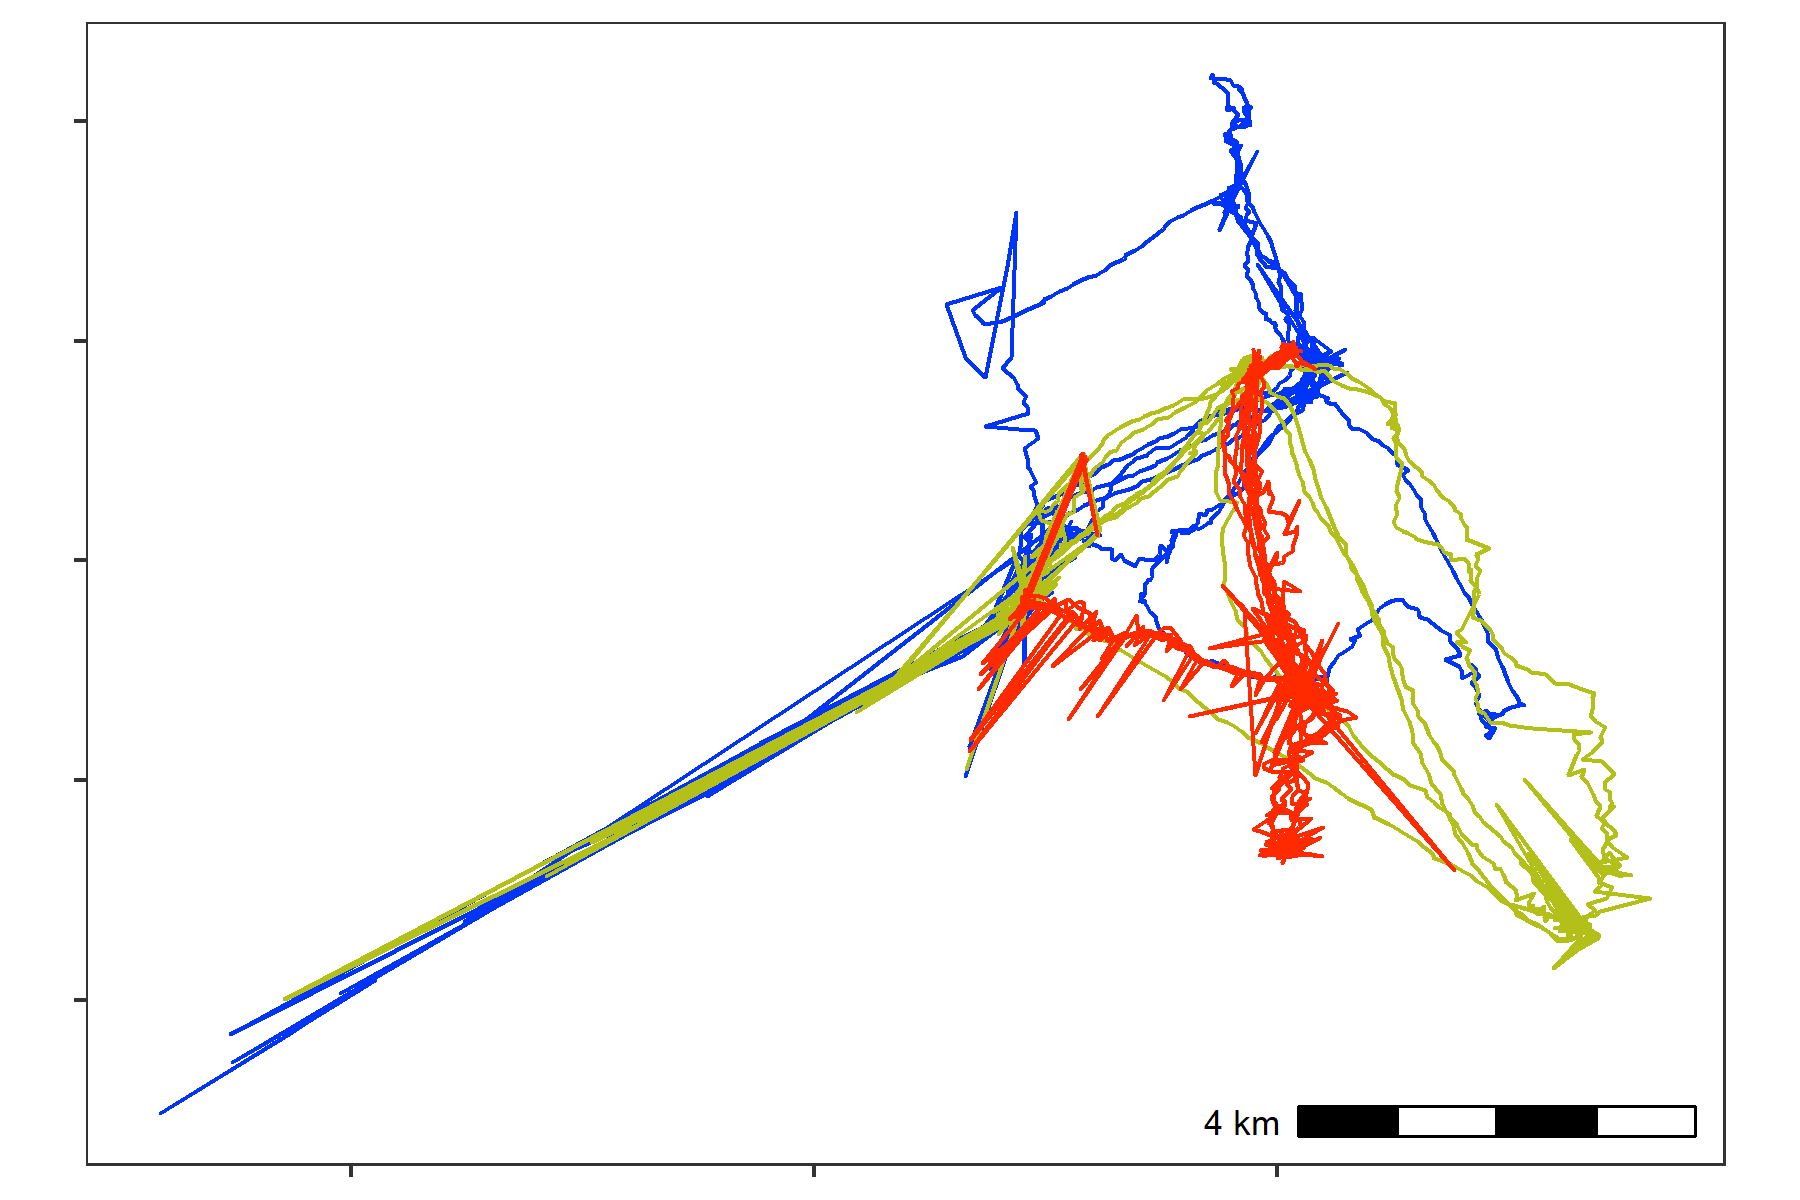
\includegraphics{figures/fig_bat_raw.png}
\caption{Movement data from three Egyptian fruit bats tracked using the ATLAS system (\emph{Rousettus aegyptiacus}; (Toledo et al. \protect\hyperlink{ref-toledo2020}{2020}; Shohami and Nathan \protect\hyperlink{ref-shohami2020}{2020})).
The bats were tracked in the Hula Valley, Israel (33.1\(^{\circ}\)N, 35.6\(^{\circ}\)E), and we use three nights of tracking (5\textsuperscript{th}, 6\textsuperscript{th}, and 7\textsuperscript{th} May, 2018), for our demonstration, with an average of 13,370 positions (SD = 2,173; range = 11,195 -- 15,542; interval = 8 seconds) per individual.
After first plotting the individual tracks, we notice severe distortions, making pre-processing necesary}
\end{figure}

\hypertarget{prepare-data-for-filtering}{%
\section{Prepare data for filtering}\label{prepare-data-for-filtering}}

Here we apply a series of simple filters.
It is always safer to deal with one individual at a time, so we split the data.table
into a list of data.tables to avoid mixups among individuals.

\hypertarget{prepare-data-per-individual}{%
\subsection{Prepare data per individual}\label{prepare-data-per-individual}}

\begin{Shaded}
\begin{Highlighting}[]
\CommentTok{# split bat data by tag}
\CommentTok{# first make a copy using the data.table function copy}
\CommentTok{# this prevents the orignal data from being modified by atlastools}
\CommentTok{# functions which DO MODIFY BY REFERENCE!}
\NormalTok{data_split <-}\StringTok{ }\KeywordTok{copy}\NormalTok{(data)}

\CommentTok{# now split}
\NormalTok{data_split <-}\StringTok{ }\KeywordTok{split}\NormalTok{(data_split, }\DataTypeTok{by =} \StringTok{"TAG"}\NormalTok{)}
\end{Highlighting}
\end{Shaded}

\hypertarget{filter-by-covariates}{%
\section{Filter by covariates}\label{filter-by-covariates}}

No natural bounds suggest themselves, so instead we proceed to filter by covariates, since point outliers are obviously visible.

We use filter out positions with \texttt{SD\ \textgreater{}\ 20} and positions calculated using only 3 base stations, using the function \texttt{atl\_filter\_covariates}.

First we calculate the variable \texttt{SD}.

\begin{Shaded}
\begin{Highlighting}[]
\CommentTok{# get SD.}
\CommentTok{# since the data are data.tables, no assignment is necessary}
\KeywordTok{invisible}\NormalTok{(}
  \KeywordTok{lapply}\NormalTok{(data_split, }\ControlFlowTok{function}\NormalTok{(dt) \{}
\NormalTok{    dt[, SD }\OperatorTok{:}\ErrorTok{=}\StringTok{ }\KeywordTok{sqrt}\NormalTok{(VARX }\OperatorTok{+}\StringTok{ }\NormalTok{VARY }\OperatorTok{+}\StringTok{ }\NormalTok{(}\DecValTok{2} \OperatorTok{*}\StringTok{ }\NormalTok{COVXY))]}
\NormalTok{  \})}
\NormalTok{)}
\end{Highlighting}
\end{Shaded}

Then we pass the filters to \texttt{atl\_filter\_covariates}.
We apply the filter to each individual's data using an \texttt{lapply}.

\begin{Shaded}
\begin{Highlighting}[]
\CommentTok{# filter for SD <= 20}
\CommentTok{# here, reassignment is necessary as rows are being removed}
\CommentTok{# the atl_filter_covariates function could have been used here}
\NormalTok{data_split <-}\StringTok{ }\KeywordTok{lapply}\NormalTok{(data_split, }\ControlFlowTok{function}\NormalTok{(dt) \{}
\NormalTok{  dt <-}\StringTok{ }\KeywordTok{atl_filter_covariates}\NormalTok{(}
    \DataTypeTok{data =}\NormalTok{ dt,}
    \DataTypeTok{filters =} \KeywordTok{c}\NormalTok{(}
      \StringTok{"SD <= 20"}\NormalTok{,}
      \StringTok{"NBS > 3"}
\NormalTok{    )}
\NormalTok{  )}
\NormalTok{\})}
\end{Highlighting}
\end{Shaded}

\hypertarget{sanity-check-plot-filtered-data}{%
\subsection{Sanity check: Plot filtered data}\label{sanity-check-plot-filtered-data}}

We plot the data to check whether the filtering has improved the data (Fig. 2.2).
The plot code is once again hidden in this rendering, but is available in the source code file.

\begin{figure}
\centering
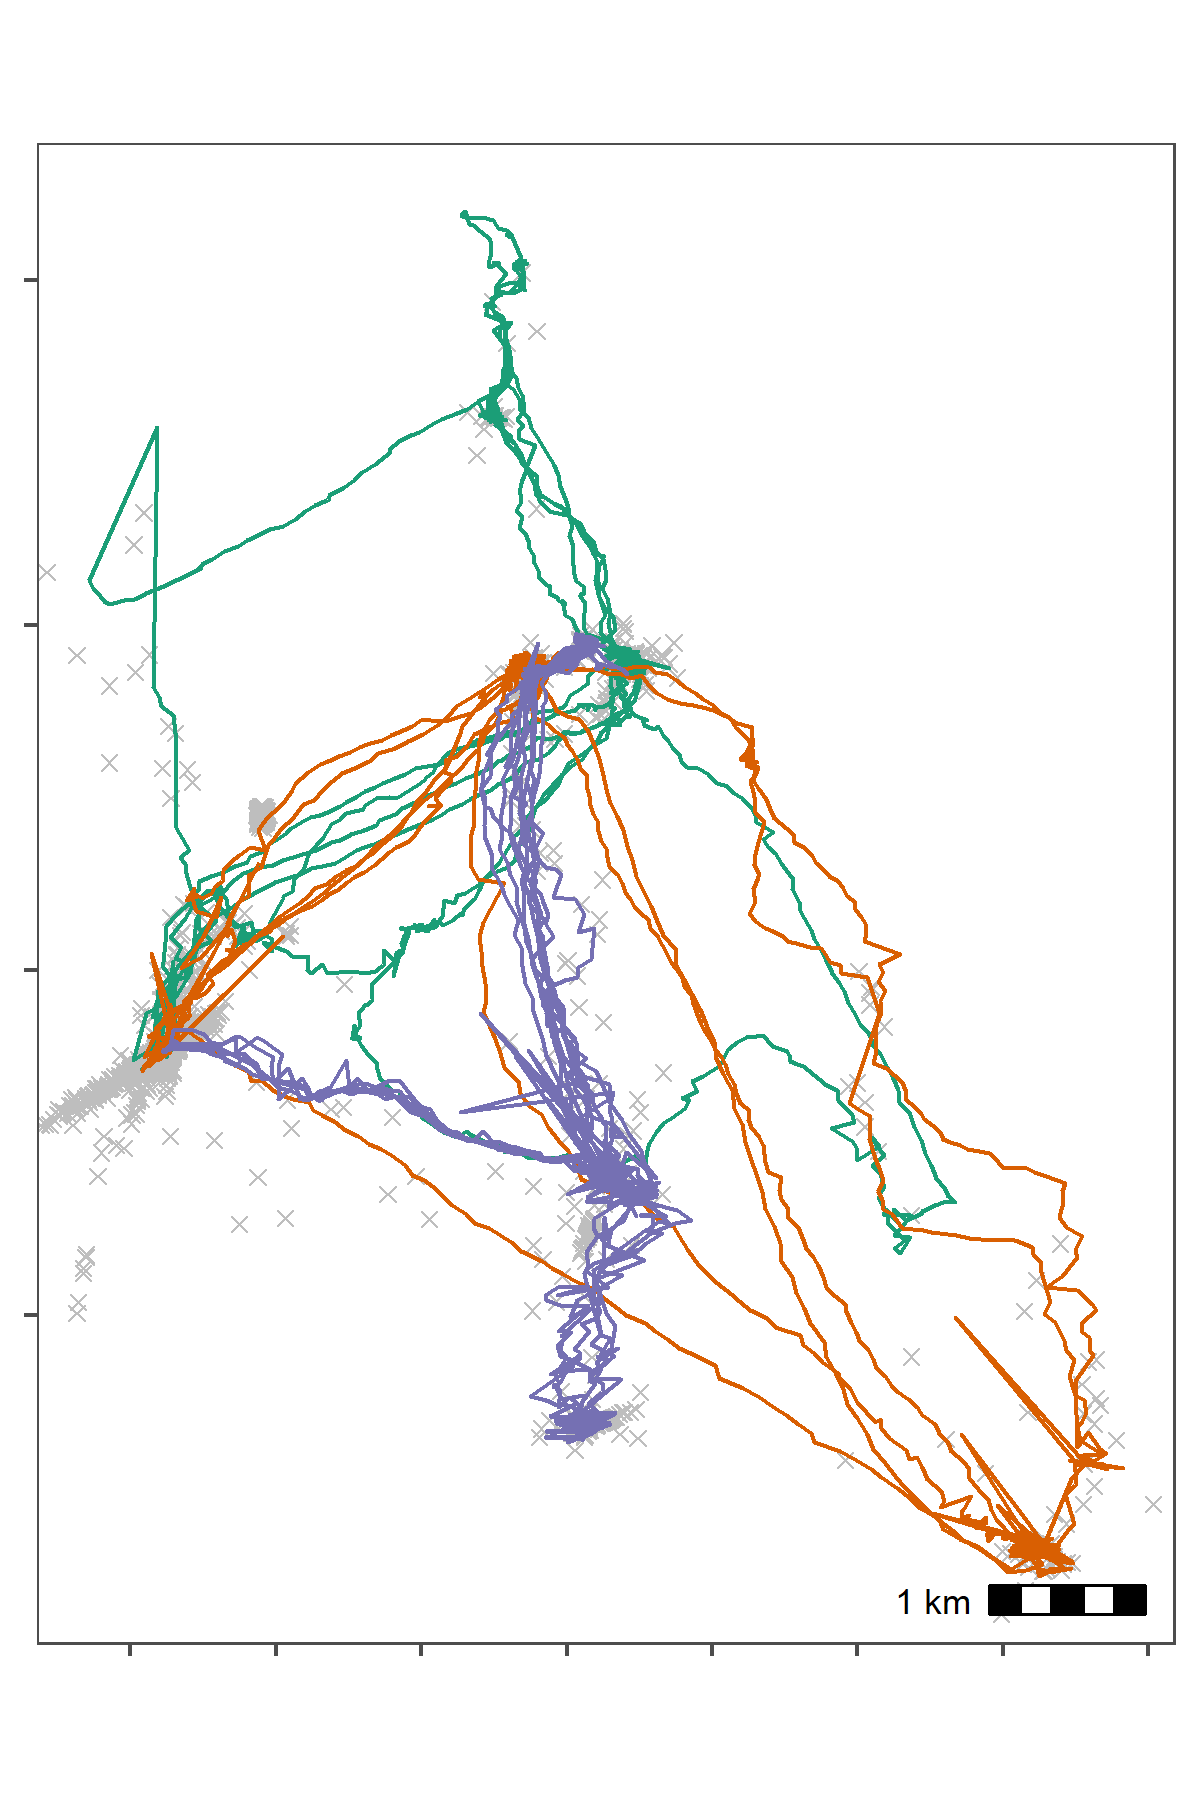
\includegraphics{figures/fig_bat_filter_cov.png}
\caption{Bat data filtered for large location errors, removing observations with standard deviation \(>\) 20. Grey crosses show data that were removed. Since the number of base stations used in the location process is a good indicator of error (Weiser et al. \protect\hyperlink{ref-weiser2016}{2016}), we also removed observations calculated using fewer than four base stations. Both steps used the function \texttt{atl\_filter\_covariates}.
This filtering reduced the data to an average of 10,447 positions per individual (78\% of the raw data on average). However, some point outliers remain.}
\end{figure}

\hypertarget{filter-by-speed}{%
\section{Filter by speed}\label{filter-by-speed}}

Some point outliers remain, and could be removed using a speed filter.

First we calculate speeds, using \texttt{atl\_get\_speed}. We must assign the speed output to a new column in the data.table, which has a special syntax which modifies in place, and is shown below. This syntax is a feature of the \texttt{data.table} package, not strictly of \texttt{atlastools} (Dowle and Srinivasan \protect\hyperlink{ref-dowle2020}{2020}).

\begin{Shaded}
\begin{Highlighting}[]
\CommentTok{# get speeds as with SD, no reassignment required for columns}
\KeywordTok{invisible}\NormalTok{(}
  \KeywordTok{lapply}\NormalTok{(data_split, }\ControlFlowTok{function}\NormalTok{(dt) \{}

    \CommentTok{# first process time to seconds}
    \CommentTok{# assign to a new column}
\NormalTok{    dt[, time }\OperatorTok{:}\ErrorTok{=}\StringTok{ }\KeywordTok{floor}\NormalTok{(TIME }\OperatorTok{/}\StringTok{ }\DecValTok{1000}\NormalTok{)]}

\NormalTok{    dt[, }\StringTok{`}\DataTypeTok{:=}\StringTok{`}\NormalTok{(}
      \DataTypeTok{speed_in =} \KeywordTok{atl_get_speed}\NormalTok{(dt,}
        \DataTypeTok{x =} \StringTok{"X"}\NormalTok{, }\DataTypeTok{y =} \StringTok{"Y"}\NormalTok{,}
        \DataTypeTok{time =} \StringTok{"time"}\NormalTok{,}
        \DataTypeTok{type =} \StringTok{"in"}
\NormalTok{      ),}
      \DataTypeTok{speed_out =} \KeywordTok{atl_get_speed}\NormalTok{(dt,}
        \DataTypeTok{x =} \StringTok{"X"}\NormalTok{, }\DataTypeTok{y =} \StringTok{"Y"}\NormalTok{,}
        \DataTypeTok{time =} \StringTok{"time"}\NormalTok{,}
        \DataTypeTok{type =} \StringTok{"out"}
\NormalTok{      )}
\NormalTok{    )]}
\NormalTok{  \})}
\NormalTok{)}
\end{Highlighting}
\end{Shaded}

Now filter for speeds \textgreater{} 20 m/s (around 70 km/h), passing the predicate (a statement return TRUE or FALSE) to \texttt{atl\_filter\_covariates}. First, we remove positions which have \texttt{NA} for their \texttt{speed\_in} (the first position) and their \texttt{speed\_out} (last position).

\begin{Shaded}
\begin{Highlighting}[]
\CommentTok{# filter speeds}
\CommentTok{# reassignment is required here}
\NormalTok{data_split <-}\StringTok{ }\KeywordTok{lapply}\NormalTok{(data_split, }\ControlFlowTok{function}\NormalTok{(dt) \{}
\NormalTok{  dt <-}\StringTok{ }\KeywordTok{na.omit}\NormalTok{(dt, }\DataTypeTok{cols =} \KeywordTok{c}\NormalTok{(}\StringTok{"speed_in"}\NormalTok{, }\StringTok{"speed_out"}\NormalTok{))}

\NormalTok{  dt <-}\StringTok{ }\KeywordTok{atl_filter_covariates}\NormalTok{(}
    \DataTypeTok{data =}\NormalTok{ dt,}
    \DataTypeTok{filters =} \KeywordTok{c}\NormalTok{(}
      \StringTok{"speed_in <= 20"}\NormalTok{,}
      \StringTok{"speed_out <= 20"}
\NormalTok{    )}
\NormalTok{  )}
\NormalTok{\})}
\end{Highlighting}
\end{Shaded}

\hypertarget{sanity-check-plot-speed-filtered-data}{%
\subsection{Sanity check: Plot speed filtered data}\label{sanity-check-plot-speed-filtered-data}}

The speed filtered data is now inspected for errors (Fig. 2.3). The plot code is once again hidden.

\begin{figure}
\centering
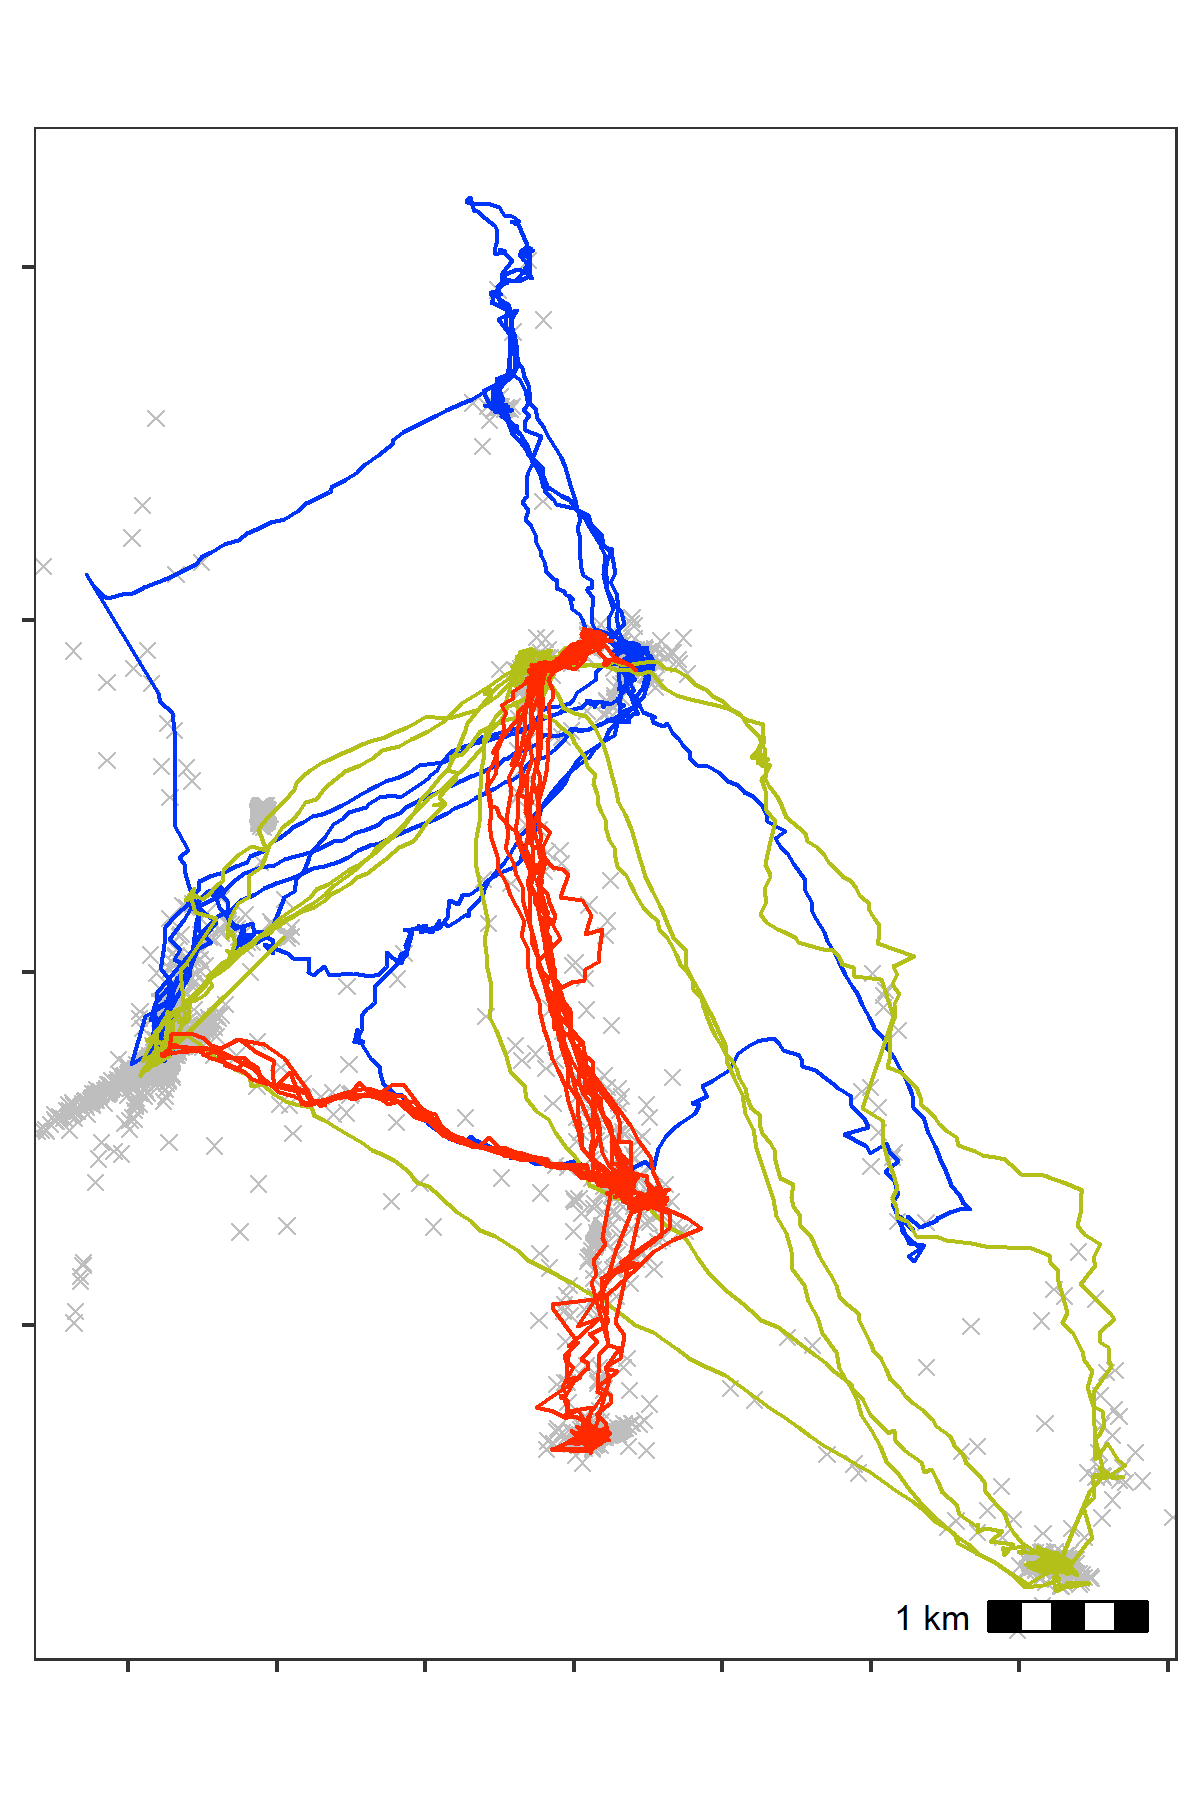
\includegraphics{figures/fig_bat_filter_speed.png}
\caption{Bat data with unrealistic speeds removed. Grey crosses show data that were removed. We calculated the incoming and outgoing speed of each position using \texttt{atl\_get\_speed}, and filtered out positions with speeds \textgreater{} 20 m/s using \texttt{atl\_filter\_covariates}, leaving 10,337 positions per individual on average (98\% from the previous step).}
\end{figure}

\hypertarget{median-smoothing}{%
\section{Median smoothing}\label{median-smoothing}}

The quality of the data is relatively high, and a median smooth is not strictly necessary. We demonstrate the application of a 5 point median smooth to the data nonetheless (Fig. 2.4).

Since the median smoothing function \texttt{atl\_median\_smooth} modifies in place, we first make a copy of the data, using \texttt{data.table}'s \texttt{copy} function.
No reassignment is required, in this case. The \texttt{lapply} function allows arguments to \texttt{atl\_median\_smooth} to be passed within \texttt{lapply} itself.

In this case, the same moving window \(K\) is applied to all individuals, but modifying this code to use the multivariate version \texttt{Map} allows different \(K\) to be used for different individuals. This is a programming matter, and is not covered here further.

\begin{Shaded}
\begin{Highlighting}[]
\CommentTok{# since the function modifies in place, we shall make a copy}
\NormalTok{data_smooth <-}\StringTok{ }\KeywordTok{copy}\NormalTok{(data_split)}

\CommentTok{# split the data again}
\NormalTok{data_smooth <-}\StringTok{ }\KeywordTok{split}\NormalTok{(data_smooth, }\DataTypeTok{by =} \StringTok{"TAG"}\NormalTok{)}
\end{Highlighting}
\end{Shaded}

\begin{Shaded}
\begin{Highlighting}[]
\CommentTok{# apply the median smooth to each list element}
\CommentTok{# no reassignment is required as THE FUNCTION MODIFIES IN PLACE!}
\KeywordTok{invisible}\NormalTok{(}

  \CommentTok{# the function arguments to atl_median_smooth}
  \CommentTok{# can be passed directly in lapply}

  \KeywordTok{lapply}\NormalTok{(}
    \DataTypeTok{X =}\NormalTok{ data_smooth,}
    \DataTypeTok{FUN =}\NormalTok{ atl_median_smooth,}
    \DataTypeTok{time =} \StringTok{"time"}\NormalTok{, }\DataTypeTok{moving_window =} \DecValTok{5}
\NormalTok{  )}
\NormalTok{)}
\end{Highlighting}
\end{Shaded}

\hypertarget{sanity-check-plot-smoothed-data}{%
\subsection{Sanity check: Plot smoothed data}\label{sanity-check-plot-smoothed-data}}

\begin{figure}
\centering
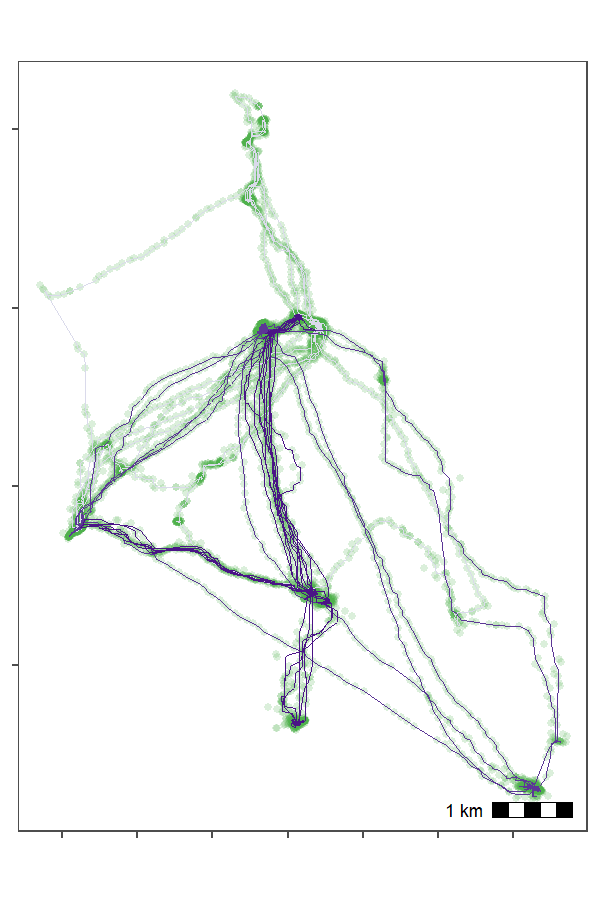
\includegraphics{figures/fig_bat_smooth.png}
\caption{Bat data after applying a median smooth with a moving window \(K\) = 5. Grey crosses show data prior to smoothing. The smoothing step did not discard any data.}
\end{figure}

\hypertarget{making-residence-patches}{%
\section{Making residence patches}\label{making-residence-patches}}

\hypertarget{calculating-residence-time}{%
\subsection{Calculating residence time}\label{calculating-residence-time}}

First, the data is put through the \texttt{recurse} package to get residence time (Bracis, Bildstein, and Mueller \protect\hyperlink{ref-bracis2018}{2018}).

\begin{Shaded}
\begin{Highlighting}[]
\CommentTok{# split the data}
\NormalTok{data_smooth <-}\StringTok{ }\KeywordTok{split}\NormalTok{(data_smooth, data_smooth}\OperatorTok{$}\NormalTok{TAG)}
\end{Highlighting}
\end{Shaded}

We calculated residence time, but since bats may revisit the same features, we want to prevent confusion between frequent revisits and prolonged residence.

For this, we stop summing residence times within \(Z\) metres of a location if the animal exited the area for one hour or more. The value of \(Z\) (radius, in \texttt{recurse} parameter terms) was chosen as 50m.

This step is relatively complicated and is only required for individuals which frequently return to the same location, or pass over the same areas repeatedly, and for which revisits (cumulative time spent) may be confused for residence time in a single visit.

While a simpler implementation using total residence time divided by the number of revisits is also possible, this does assume that each revisit had the same residence time.

\begin{Shaded}
\begin{Highlighting}[]
\CommentTok{# get residence times}

\NormalTok{data_residence <-}\StringTok{ }\KeywordTok{lapply}\NormalTok{(data_smooth, }\ControlFlowTok{function}\NormalTok{(dt) \{}
  \CommentTok{# do basic recurse}
\NormalTok{  dt_recurse <-}\StringTok{ }\KeywordTok{getRecursions}\NormalTok{(}
    \DataTypeTok{x =}\NormalTok{ dt[, }\KeywordTok{c}\NormalTok{(}\StringTok{"X"}\NormalTok{, }\StringTok{"Y"}\NormalTok{, }\StringTok{"time"}\NormalTok{, }\StringTok{"TAG"}\NormalTok{)],}
    \DataTypeTok{radius =} \DecValTok{50}\NormalTok{,}
    \DataTypeTok{timeunits =} \StringTok{"mins"}
\NormalTok{  )}

  \CommentTok{# get revisit stats}
\NormalTok{  dt_recurse <-}\StringTok{ }\KeywordTok{setDT}\NormalTok{(}
\NormalTok{    dt_recurse[[}\StringTok{"revisitStats"}\NormalTok{]]}
\NormalTok{  )}

  \CommentTok{# count long absences from the area}
\NormalTok{  dt_recurse[, timeSinceLastVisit }\OperatorTok{:}\ErrorTok{=}
\StringTok{    }\KeywordTok{ifelse}\NormalTok{(}\KeywordTok{is.na}\NormalTok{(timeSinceLastVisit), }\OperatorTok{-}\OtherTok{Inf}\NormalTok{, timeSinceLastVisit)]}
\NormalTok{  dt_recurse[, longAbsenceCounter }\OperatorTok{:}\ErrorTok{=}\StringTok{ }\KeywordTok{cumsum}\NormalTok{(timeSinceLastVisit }\OperatorTok{>}\StringTok{ }\DecValTok{60}\NormalTok{),}
\NormalTok{    by =}\StringTok{ }\NormalTok{.(coordIdx)}
\NormalTok{  ]}
  \CommentTok{# get data before the first long absence of 60 mins}
\NormalTok{  dt_recurse <-}\StringTok{ }\NormalTok{dt_recurse[longAbsenceCounter }\OperatorTok{<}\StringTok{ }\DecValTok{1}\NormalTok{, ]}

\NormalTok{  dt_recurse <-}\StringTok{ }\NormalTok{dt_recurse[, }\KeywordTok{list}\NormalTok{(}
    \DataTypeTok{resTime =} \KeywordTok{sum}\NormalTok{(timeInside),}
    \DataTypeTok{fpt =} \KeywordTok{first}\NormalTok{(timeInside),}
    \DataTypeTok{revisits =} \KeywordTok{max}\NormalTok{(visitIdx)}
\NormalTok{  ),}
\NormalTok{  by =}\StringTok{ }\NormalTok{.(coordIdx, x, y)}
\NormalTok{  ]}

  \CommentTok{# prepare and merge existing data with recursion data}
\NormalTok{  dt[, coordIdx }\OperatorTok{:}\ErrorTok{=}\StringTok{ }\KeywordTok{seq}\NormalTok{(}\KeywordTok{nrow}\NormalTok{(dt))]}

\NormalTok{  dt <-}\StringTok{ }\KeywordTok{merge}\NormalTok{(dt,}
\NormalTok{    dt_recurse[, }\KeywordTok{c}\NormalTok{(}\StringTok{"coordIdx"}\NormalTok{, }\StringTok{"resTime"}\NormalTok{)],}
    \DataTypeTok{by =} \KeywordTok{c}\NormalTok{(}\StringTok{"coordIdx"}\NormalTok{)}
\NormalTok{  )}

  \KeywordTok{setorderv}\NormalTok{(dt, }\StringTok{"time"}\NormalTok{)}
\NormalTok{\})}
\end{Highlighting}
\end{Shaded}

We bind the data together and assign a human readable timestamp column.

\begin{Shaded}
\begin{Highlighting}[]
\CommentTok{# bind the list}
\NormalTok{data_residence <-}\StringTok{ }\KeywordTok{rbindlist}\NormalTok{(data_residence)}

\CommentTok{# get time as human readable}
\NormalTok{data_residence[, ts }\OperatorTok{:}\ErrorTok{=}\StringTok{ }\KeywordTok{as.POSIXct}\NormalTok{(time, }\DataTypeTok{origin =} \StringTok{"1970-01-01"}\NormalTok{)]}
\end{Highlighting}
\end{Shaded}

\hypertarget{constructing-residence-patches}{%
\subsection{Constructing residence patches}\label{constructing-residence-patches}}

Some preparation is required. First, the function requires columns \texttt{x}, \texttt{y},
\texttt{time}, and \texttt{id}, which we assign using the \texttt{data.table} syntax.
Then we subset the data to only work with positions where the individual had a residence time of more than 5 minutes.

\begin{Shaded}
\begin{Highlighting}[]
\CommentTok{# add an id column}
\NormalTok{data_residence[, }\StringTok{`}\DataTypeTok{:=}\StringTok{`}\NormalTok{(}
  \DataTypeTok{id =}\NormalTok{ TAG,}
  \DataTypeTok{x =}\NormalTok{ X, }\DataTypeTok{y =}\NormalTok{ Y}
\NormalTok{)]}

\CommentTok{# filter for residence time > 5 minutes}
\NormalTok{data_residence <-}\StringTok{ }\NormalTok{data_residence[resTime }\OperatorTok{>}\StringTok{ }\DecValTok{5}\NormalTok{, ]}

\CommentTok{# split the data}
\NormalTok{data_residence <-}\StringTok{ }\KeywordTok{split}\NormalTok{(data_residence, data_residence}\OperatorTok{$}\NormalTok{TAG)}
\end{Highlighting}
\end{Shaded}

We apply the residence patch method, using the default argument values (\texttt{lim\_spat\_indep\ =\ 100} (metres), \texttt{lim\_time\_indep\ =\ 30} (minutes), and \texttt{min\_fixes\ =\ 3}). We change the \texttt{buffer\_radius} to 25 metres (twice the buffer radius is used, so points must be separated by 50m to be independent bouts).

\begin{Shaded}
\begin{Highlighting}[]
\CommentTok{# segment into residence patches}
\NormalTok{data_patches <-}\StringTok{ }\KeywordTok{lapply}\NormalTok{(data_residence, atl_res_patch,}
  \DataTypeTok{buffer_radius =} \DecValTok{25}
\NormalTok{)}
\end{Highlighting}
\end{Shaded}

\hypertarget{getting-residence-patch-data}{%
\subsection{Getting residence patch data}\label{getting-residence-patch-data}}

We extract the residence patch data as spatial \texttt{sf-MULTIPOLYGON} objects.
These are returned as a list and must be converted into a single \texttt{sf} object.
These objects and the raw movement data are shown in Fig. 2.5.

\begin{Shaded}
\begin{Highlighting}[]
\CommentTok{# get data spatials}
\NormalTok{data_spatials <-}\StringTok{ }\KeywordTok{lapply}\NormalTok{(data_patches, atl_patch_summary,}
  \DataTypeTok{which_data =} \StringTok{"spatial"}\NormalTok{,}
  \DataTypeTok{buffer_radius =} \DecValTok{25}
\NormalTok{)}

\CommentTok{# bind list}
\NormalTok{data_spatials <-}\StringTok{ }\KeywordTok{rbindlist}\NormalTok{(data_spatials)}

\CommentTok{# convert to sf}
\KeywordTok{library}\NormalTok{(sf)}
\NormalTok{data_spatials <-}\StringTok{ }\KeywordTok{st_sf}\NormalTok{(data_spatials, }\DataTypeTok{sf_column_name =} \StringTok{"polygons"}\NormalTok{)}

\CommentTok{# assign a crs}
\KeywordTok{st_crs}\NormalTok{(data_spatials) <-}\StringTok{ }\KeywordTok{st_crs}\NormalTok{(}\DecValTok{2039}\NormalTok{)}
\end{Highlighting}
\end{Shaded}

\hypertarget{write-patch-spatial-representations}{%
\subsection{Write patch spatial representations}\label{write-patch-spatial-representations}}

\begin{Shaded}
\begin{Highlighting}[]
\KeywordTok{st_write}\NormalTok{(data_spatials,}
  \DataTypeTok{dsn =} \StringTok{"data/data_bat_residence_patches.gpkg"}
\NormalTok{)}
\end{Highlighting}
\end{Shaded}

Write cleaned bat data.

\begin{Shaded}
\begin{Highlighting}[]
\KeywordTok{fwrite}\NormalTok{(}\KeywordTok{rbindlist}\NormalTok{(data_smooth),}
  \DataTypeTok{file =} \StringTok{"data/data_bat_smooth.csv"}
\NormalTok{)}
\end{Highlighting}
\end{Shaded}

Write patch summary.

\begin{Shaded}
\begin{Highlighting}[]
\CommentTok{# get summary}
\NormalTok{patch_summary <-}\StringTok{ }\KeywordTok{lapply}\NormalTok{(data_patches, atl_patch_summary)}

\CommentTok{# bind summary}
\NormalTok{patch_summary <-}\StringTok{ }\KeywordTok{rbindlist}\NormalTok{(patch_summary)}

\CommentTok{# write}
\KeywordTok{fwrite}\NormalTok{(}
\NormalTok{  patch_summary,}
  \StringTok{"data/data_bat_patch_summary.csv"}
\NormalTok{)}
\end{Highlighting}
\end{Shaded}

\begin{figure}
\centering
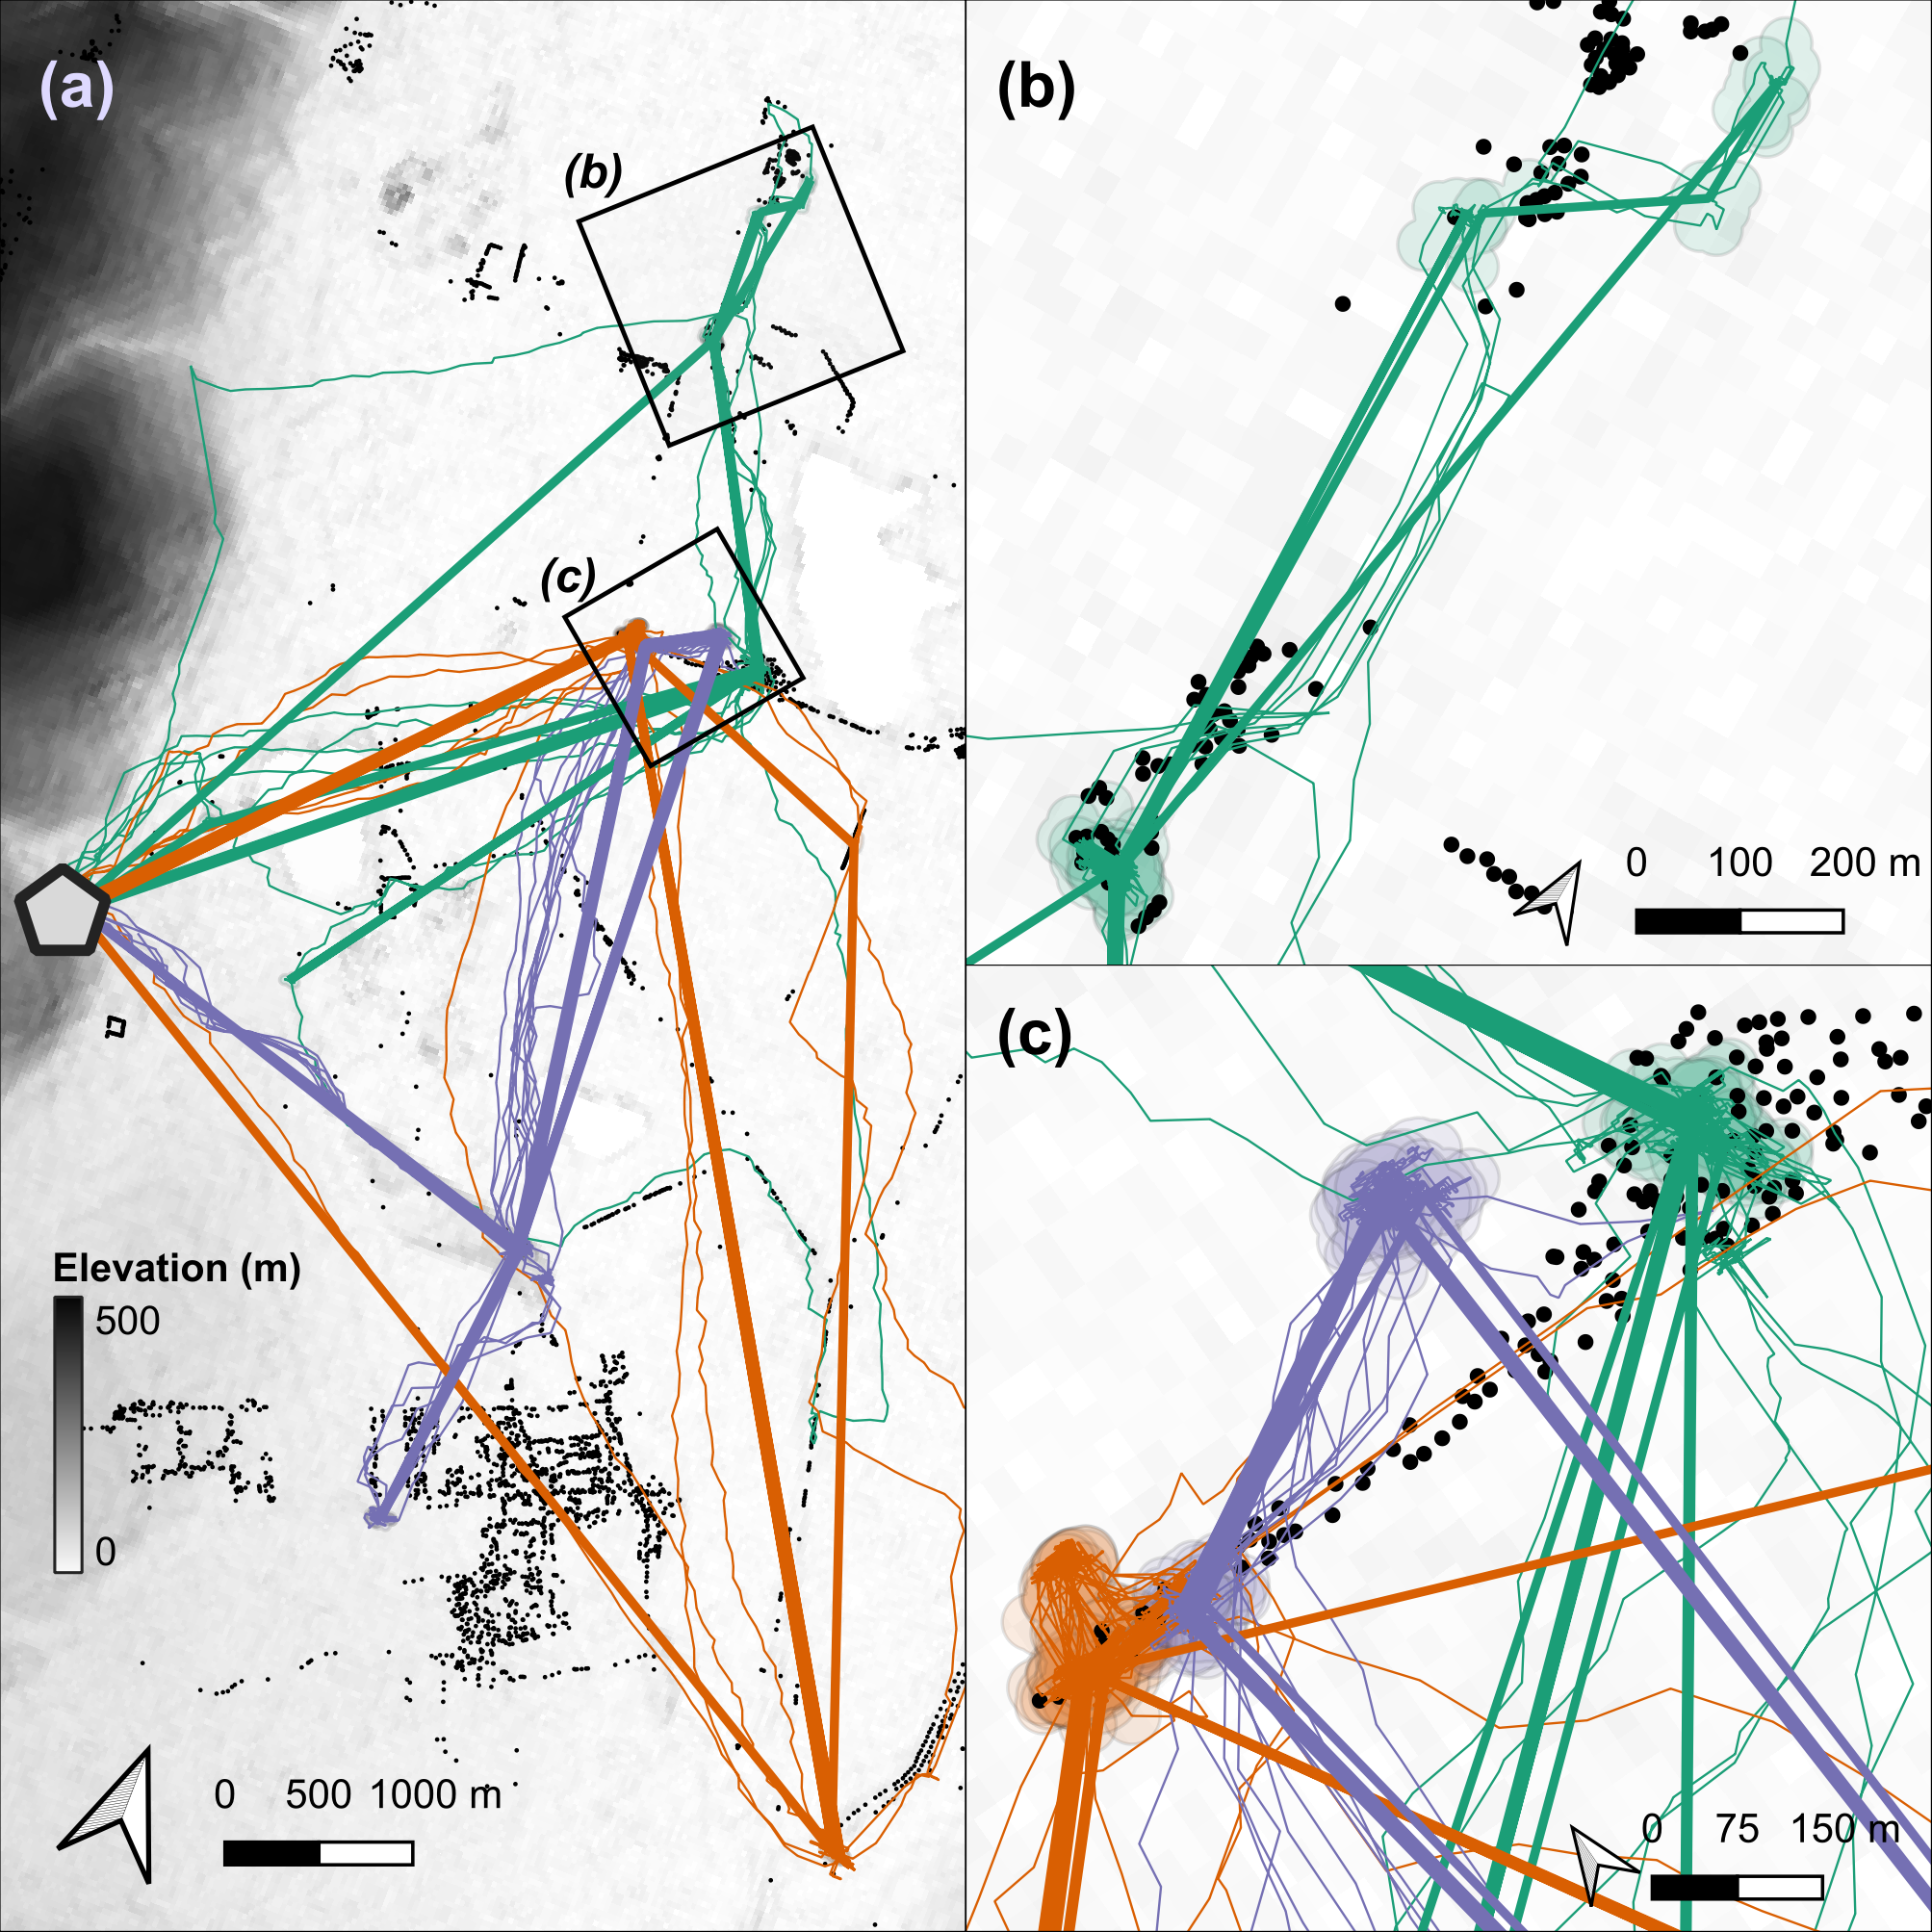
\includegraphics{figures/fig_07_bats.png}
\caption{A visual examination of plots of the bats' residence patches and linear approximations of paths between them showed that though all three bats roosted at the same site, they used distinct areas of the study site over the three nights \textbf{(a)}.
Bats tended to be resident near fruit trees, which are their main food source, travelling repeatedly between previously visited areas \textbf{(b, c)}.
However, bats also appeared to spend some time at locations where no fruit trees were recorded, prompting questions about their use of other food sources \textbf{(b, c)}.
When bats did occur close together, their residence patches barely overlapped, and their paths to and from the broad area of co-occurrence were not similar \textbf{(c)}.
Constructing residence patches for multiple individuals over multiple activity periods suggests interesting dynamics of within- and between-individual overlap \textbf{(b, c)}.}
\end{figure}

\hypertarget{references}{%
\chapter{References}\label{references}}

\hypertarget{refs}{}
\leavevmode\hypertarget{ref-barraquand2008}{}%
Barraquand, Frédéric, and Simon Benhamou. 2008. ``Animal Movements in Heterogeneous Landscapes: Identifying Profitable Places and Homogeneous Movement Bouts.'' \emph{Ecology} 89 (12): 3336--48. \url{https://doi.org/10.1890/08-0162.1}.

\leavevmode\hypertarget{ref-bijleveld2016}{}%
Bijleveld, Allert Imre, Robert B MacCurdy, Ying-Chi Chan, Emma Penning, Richard M. Gabrielson, John Cluderay, Erik L. Spaulding, et al. 2016. ``Understanding Spatial Distributions: Negative Density-Dependence in Prey Causes Predators to Trade-Off Prey Quantity with Quality.'' \emph{Proceedings of the Royal Society B: Biological Sciences} 283 (1828): 20151557. \url{https://doi.org/10.1098/rspb.2015.1557}.

\leavevmode\hypertarget{ref-bracis2018}{}%
Bracis, Chloe, Keith L. Bildstein, and Thomas Mueller. 2018. ``Revisitation Analysis Uncovers Spatio-Temporal Patterns in Animal Movement Data.'' \emph{Ecography} 41 (11): 1801--11. \url{https://doi.org/10.1111/ecog.03618}.

\leavevmode\hypertarget{ref-dowle2020}{}%
Dowle, Matt, and Arun Srinivasan. 2020. \emph{Data.Table: Extension of `data.Frame`}. Manual.

\leavevmode\hypertarget{ref-gupte2020a}{}%
Gupte, Pratik Rajan. 2020. ``Atlastools: Pre-Processing Tools for High Frequency Tracking Data.'' Zenodo. \url{https://doi.org/10.5281/ZENODO.4033154}.

\leavevmode\hypertarget{ref-oudman2018}{}%
Oudman, Thomas, Theunis Piersma, Mohamed V. Ahmedou Salem, Marieke E. Feis, Anne Dekinga, Sander Holthuijsen, Job ten Horn, Jan A. van Gils, and Allert I. Bijleveld. 2018. ``Resource Landscapes Explain Contrasting Patterns of Aggregation and Site Fidelity by Red Knots at Two Wintering Sites.'' \emph{Movement Ecology} 6 (1): 24--24. \url{https://doi.org/10.1186/s40462-018-0142-4}.

\leavevmode\hypertarget{ref-shohami2020}{}%
Shohami, David, and Ran Nathan. 2020. ``Cognitive Map-Based Navigation in Wild Bats Revealed by a New High-Throughput Tracking System.'' Dryad. \url{https://doi.org/10.5061/DRYAD.G4F4QRFN2}.

\leavevmode\hypertarget{ref-toledo2020}{}%
Toledo, Sivan, David Shohami, Ingo Schiffner, Emmanuel Lourie, Yotam Orchan, Yoav Bartan, and Ran Nathan. 2020. ``Cognitive MapBased Navigation in Wild Bats Revealed by a New High-Throughput Tracking System.'' \emph{Science} 369 (6500): 188--93. \url{https://doi.org/10.1126/science.aax6904}.

\leavevmode\hypertarget{ref-weiser2016}{}%
Weiser, Adi Weller, Yotam Orchan, Ran Nathan, Motti Charter, Anthony J. Weiss, and Sivan Toledo. 2016. ``Characterizing the Accuracy of a Self-Synchronized Reverse-GPS Wildlife Localization System.'' In \emph{2016 15th ACM/IEEE International Conference on Information Processing in Sensor Networks (IPSN)}, 1--12. \url{https://doi.org/10.1109/IPSN.2016.7460662}.

\end{document}
